%% Plantilla CAS-SC (Elsevier) -- doble columna
%% Adaptado para: Expert Systems with Applications
%% Manuscrito original en formato Springer LLNCS, convertido a UTF-8.

\documentclass[a4paper,fleqn]{cas-sc}

% Bibliografía estilo nombre-año (compatible con cas-model2-names)
\usepackage[authoryear,longnamesfirst]{natbib}
\usepackage{stfloats}

% Codificación y tipografía
\usepackage[utf8]{inputenc}
\usepackage[T1]{fontenc}

% Paquetes usados en el cuerpo del artículo
\usepackage{amsmath,amssymb}
\usepackage{array}
\usepackage{booktabs}
\usepackage{multirow}
\usepackage{adjustbox}
\usepackage{wrapfig}
\usepackage{float}
\usepackage{verbatim}
\usepackage{eurosym}

\begin{document}
\let\WriteBookmarks\relax
\def\floatpagepagefraction{1}
\def\textpagefraction{.001}

% Título corto (encabezado)
\shorttitle{Análisis de licitaciones públicas con sistemas de reglas}

% Autores cortos (encabezado)
\shortauthors{M.F. Molina-Miranda et~al.}

% Título principal
\title[mode=title]{Análisis de licitaciones públicas con Sistemas de Reglas para mejorar la toma de decisiones}

% Nota de financiación / agradecimientos
\tnotemark[1]
\tnotetext[1]{This work is based on the results of the research project conducted at the Universidad de Guayaquil, entitled: ``\textit{Prediction model for improving decision-making in public tender recommendation systems incorporating explainable artificial intelligence techniques}''.}

%==================== AUTORES ====================
\author[1,2]{Maria Fernanda Molina-Miranda}[orcid=0000-0000-0000-0000]
\cormark[1]
\fnmark[1]
\ead{maria.molinam@ug.edu.ec}

\author[1]{Angel Cuenca-Ortega}
\ead{angel.cuencao@ug.edu.ec}

\author[2]{Juan Fernandez-Olivares}
\ead{faro@decsai.ugr.es}

\author[2]{Raul Pérez}
\ead{fgr@decsai.ugr.es}

%==================== AFILIACIONES ====================
\affiliation[1]{organization={Universidad de Guayaquil, FCMF},
            city={Guayaquil},
            country={Ecuador}}

\affiliation[2]{organization={Universidad de Granada, DECSAI},
            city={Granada},
            country={Spain}}

% Autor de correspondencia
\cortext[1]{Corresponding author}

%==================== RESUMEN ====================
\begin{abstract}
Este estudio presenta una metodología integral para evaluar y comparar el rendimiento de modelos de clasificación supervisada aplicados a licitaciones públicas en el contexto de la Unión Europea. El enfoque propuesto combina los algoritmos Random Forest y Gradient Boosting con técnicas de inteligencia artificial explicable (XAI) y un sistema de reglas, con el objetivo de apoyar la optimización del proceso de adjudicación mediante la identificación de patrones históricos asociados a decisiones favorables. A partir de datos públicos provenientes de la plataforma TED, se construyó un conjunto de datos normalizado mediante un proceso ETL escalable basado en Apache Spark, seguido de un análisis exploratorio y un modelado multiclase alineado con la Metodología Fundamental para la Ciencia de Datos. Los modelos fueron evaluados utilizando matrices de confusión y métricas agregadas de clasificación, incluyendo accuracy, precision, recall y F1-score, lo que permitió una comparación objetiva de su desempeño y estabilidad. Los resultados muestran un rendimiento competitivo de ambos modelos, con una ligera ventaja de Gradient Boosting en escenarios de mayor complejidad, pero con mayor costo computacional. La integración de explicaciones locales mediante LIME y reglas interpretables mejora la transparencia de las predicciones y facilita su uso en contextos donde la trazabilidad es un requisito crítico.
\end{abstract}

%==================== HIGHLIGHTS ====================
% Revisar/editar: ESWA pide 3-5 highlights de <=85 caracteres.
\begin{highlights}
\item Metodología reproducible para clasificar licitaciones públicas europeas (datos TED).
\item Comparación de Random Forest y Gradient Boosting con validación cruzada (k=10).
\item Integración de XAI (LIME) y reglas if-then para explicar las predicciones.
\item Random Forest supera a Gradient Boosting en F1-macro y AUC con menor costo.
\end{highlights}

%==================== PALABRAS CLAVE ====================
\begin{keywords}
Licitaciones públicas \sep Aprendizaje automático \sep Random Forest \sep Gradient Boosting \sep Inteligencia artificial explicable (XAI) \sep LIME \sep Sistema de reglas
\end{keywords}

\maketitle

\section{Introduction}
\label{sec:introduction}


Una licitación, o concurso público, es un proceso donde muchos proveedores ofrecen servicios, bienes y suministros. Además, las licitaciones son consideradas también  un instrumento muy valioso y diverso para  promover la innovación, el desarrollo de \textit{pequeñas y medianas empresas} (pymes) y la sostenibilidad ambiental o social. Los contratos de las licitaciones se adjudican priorizando la oferta que mejor satisfaga los requisitos del gobierno, generalmente en función del menor costo financiero. No obstante, la adjudicación de estos contratos implica la revisión de extensos documentos por parte de múltiples asesores, lo que  convierte esta etapa en un punto crítico que, si no se gestiona de manera eficiente,  puede derivar en  pérdidas financieras \cite{IsabelGallego2021,Hoekman2024}. 

Por ello, muchos países destinan gran parte de su presupuesto a las compras públicas para garantizar la contratación del proveedor idóneo, bajo los criterios de mejor servicio, bien o ejecución de obras públicas. En el caso de los  países miembros de la Unión Europea, la inversión en compras públicas representa aproximadamente el 14 \% de su  PIB; es decir, alrededor de 2 billones de euros en total \cite{garciarodriguez2022}.  

	En los Estados miembros de la Unión Europea, las licitaciones públicas que superan los umbrales establecidos por la normativa comunitaria se publican en el Diario Oficial de la Unión Europea (DOUE), específicamente en la plataforma TED (\textit{Tenders Electronic Daily}). Esta base de datos reúne anualmente más de 500.000 anuncios de licitaciones, disponibles en las 24 lenguas oficiales de la Unión Europea, lo que facilita la participación de empresas de todos los países miembros. Debido a este elevado volumen de convocatorias, la competencia resulta particularmente intensa, con la intervención simultánea de entidades de múltiples sectores y nacionalidades.

 %
Dado el alto volumen de información y la necesidad de optimizar la toma de decisiones, el uso de herramientas basadas en modelos de \textit{Machine Learning} (ML) se ha convertido en una estrategia fundamental.
Estas herramientas permiten mejorar la clasificación y selección de proveedores mediante la recolección,  análisis de datos y un posterior entrenamiento adecuado de los modelos. 
%
Donde, los datos de las licitaciones adjudicadas se almacenan en archivos planos estructurados y organizados según criterios de separación entre campos. Estos archivos se encuentran respaldados en repositorios de acceso público para garantizar la transparencia de todo el proceso de licitación y pueden ser utilizados con fines analíticos, sirviendo como base para alimentar y mejorar los modelos de clasificación \cite{IsabelGallego2021}. 


	A pesar de los avances, 
	las pymes enfrentan serias limitaciones para participar en licitaciones públicas, principalmente debido a la falta de recursos técnicos y humanos que les permitan identificar a tiempo las oportunidades más viables. 
	Esta situación genera una barrera estructural de entrada, lo que lleva a que exista una baja participación de este sector en los procesos de contratación estatal. 
	%
	Para abordar esta problemática, el presente trabajo propone 
	el desarrollo de un sistema de recomendación basado en técnicas de \textit{Explainable Artificial Intelligence} (XAI), que analiza datos reales de licitaciones históricas para identificar las condiciones bajo las cuales se han adjudicado contratos. 
	%
	De esta manera, se busca ofrecer a las pymes una herramienta que les ayude a anticipar escenarios y tomar decisiones estratégicas basadas en evidencia, incrementando así sus posibilidades de competir en igualdad de condiciones en el mercado público.

\paragraph{\bf Our contribution.}

Este estudio propone una metodología para evaluar y comparar el rendimiento de los modelos de clasificación \textit{Random Forest} y \textit{Gradient Boosting}, integrando técnicas de \textit{Explainable Artificial Intelligence} 
(XAI) y sistemas de reglas. La finalidad es apoyar la optimización del proceso de adjudicación de licitaciones en países de la Unión Europea, mediante la identificación de condiciones históricas que han favorecido determinadas adjudicaciones. El enfoque permite sugerir posibles escenarios favorables para nuevas licitaciones que cumplan con parámetros similares. Además, los resultados son analizados y visualizados a través de métricas de clasificación y matrices de confusión multiclase, lo que facilita una evaluación comparativa exhaustiva del desempeño de ambos modelos.


	\section{Marco teórico}
	
%\dorevisar{
	El conjunto de datos del TED constituye una fuente de información fundamental para el análisis empírico de la contratación pública europea. 
	%
	Este repositorio integra miles de registros estructurados con un gran número de variables descriptivas sobre las entidades contratantes, los procedimientos y los resultados de adjudicación. 
	%

Cada registro incluye información estructurada en distintos niveles:
\textit{notice} (aviso general del procedimiento), el nivel \textit{lot} (lotes o secciones específicas del contrato) y el nivel \textit{contract award} (adjudicación del contrato).
Entre las variables más relevantes se incluyen 
\texttt{CAE\_TYPE}, que identifica el tipo de autoridad contratante; 
\texttt{MAIN\_ACTIVITY}, que especifica el sector de actividad principal de la entidad; 
\texttt{TYPE\_OF\_CONTRACT}, que distingue entre contratos de obras, servicios o suministros; \texttt{DURATION}, que representa la duración del contrato en meses; 
y \texttt{VALUE\_EURO}, que expresa su valor en euros sin IVA.

	Dentro de las variables consideradas, \texttt{MAIN\_ACTIVITY} es fundamental, ya que proporciona información sobre las principales áreas de actividad económica de las entidades contratantes y los valores promedio asociados a cada tipo de licitación.  Esta característica permite orientar a las pymes hacia los sectores donde su participación resulta más viable y con montos contractuales acordes a su capacidad operativa.

	Asimismo, se registran atributos como el número de contrato, la cantidad de ofertas, la identificación de pymes, las modalidades de contratación y las entidades regulatorias intervinientes. Estos campos permiten un análisis estructurado y comparativo de los procesos de adjudicación, contribuyendo a una comprensión más profunda de las condiciones y dinámicas del mercado público europeo.

En la literatura reciente, diversos estudios han abordado la clasificación en el ámbito de las licitaciones públicas mediante el uso de distintos modelos de aprendizaje automático, 
incluyendo redes neuronales. En este sentido,  la selección del algoritmo adecuado  es fundamental para la creación del modelo, ya que una elección inadecuada podría afectar la precisión de los resultados y llevar a conclusiones poco fiables. Por ejemplo, en \cite{NavasLoro2022} se presenta un clasificador de textos basado en el vocabulario común de contratación pública, con el objetivo de abordar la falta de un criterio uniforme en las adjudicaciones. Los resultados del estudio demuestran que los modelos de clasificación con mayor precisión fueron: 
\textit{Random Forest}, % (RF), 
con una precisión de 0.51; 
\textit{Decision Trees}, % (DT), 
con una precisión de 0.60 y 
\textit{Support Vector Machines}, %(SVM),  
con una precisión de 0.69.  
De manera similar, el estudio de \cite{FigueroaGomez2024} analiza la efectividad de algoritmos como 
Logistic Regression, Decision Trees, Random Forest, Gradient Boosting y AdaBoost, 
con el propósito de mejorar la clasificación de licitaciones y evaluar distintos métodos de balanceo de datos. Los resultados resaltan la superioridad de \textit{Random Forest} y \textit{Gradient Boosting} cuando se combina con técnicas de balanceo como SMOTE-TOMEK. En el presente trabajo se empleó \texttt{RandomOverSampler} como método de sobremuestreo, preferido sobre SMOTE por la presencia de variables binarias codificadas mediante \textit{OneHotEncoder} \cite{geron2019hands}.


Por otra parte, diversos estudios han resaltado la importancia de la 
 XAI en problemas donde se busca generar confianza del usuario en la toma de decisiones. 
En vista que, usualmente la complejidad de los modelos de ML son de caja negra lo que dificulta la interpretación de sus resultados. Sin embargo, al usar técnicas de XAI se puede extraer explicaciones de las clasificaciones y generar conclusiones más comprensibles que imitan el comportamiento del sistema original \cite{upm71271}. 

Para lograr esta integración, el uso de la \textit{artificial inteligence} (AI) en las contrataciones públicas  requiere  tener conocimiento de tres áreas: 
\textit{estadística}, para la correcta interpretación y modelado de datos; \textit{programación}, para la implementación y optimización de algoritmos; y \textit{normativa europea de contratación pública}, para garantizar la adecuación legal del proceso \cite{GarciaRodriguezArosa2021,garciarodriguez2022}.	
	
 
\paragraph{\bf Plan of the paper.}
El resto del artículo está organizado como sigue. En la Sección~3 se describe la metodología propuesta, organizada conforme a la Metodología Fundamental para la Ciencia de Datos, abarcando las fases de requisitos de datos, recolección, comprensión, preparación, modelado, evaluación, despliegue y retroalimentación. La Sección~4 expone y discute los resultados experimentales obtenidos con los modelos \textit{Random Forest} y \textit{Gradient Boosting}, incluyendo métricas de desempeño, matrices de confusión y análisis de explicabilidad mediante técnicas XAI. Finalmente, la Sección~5 presenta las conclusiones del estudio y plantea líneas de trabajo futuro.

	\section{Metodología}\label{sec:método}
	
\begin{figure}[t]
	\centering
	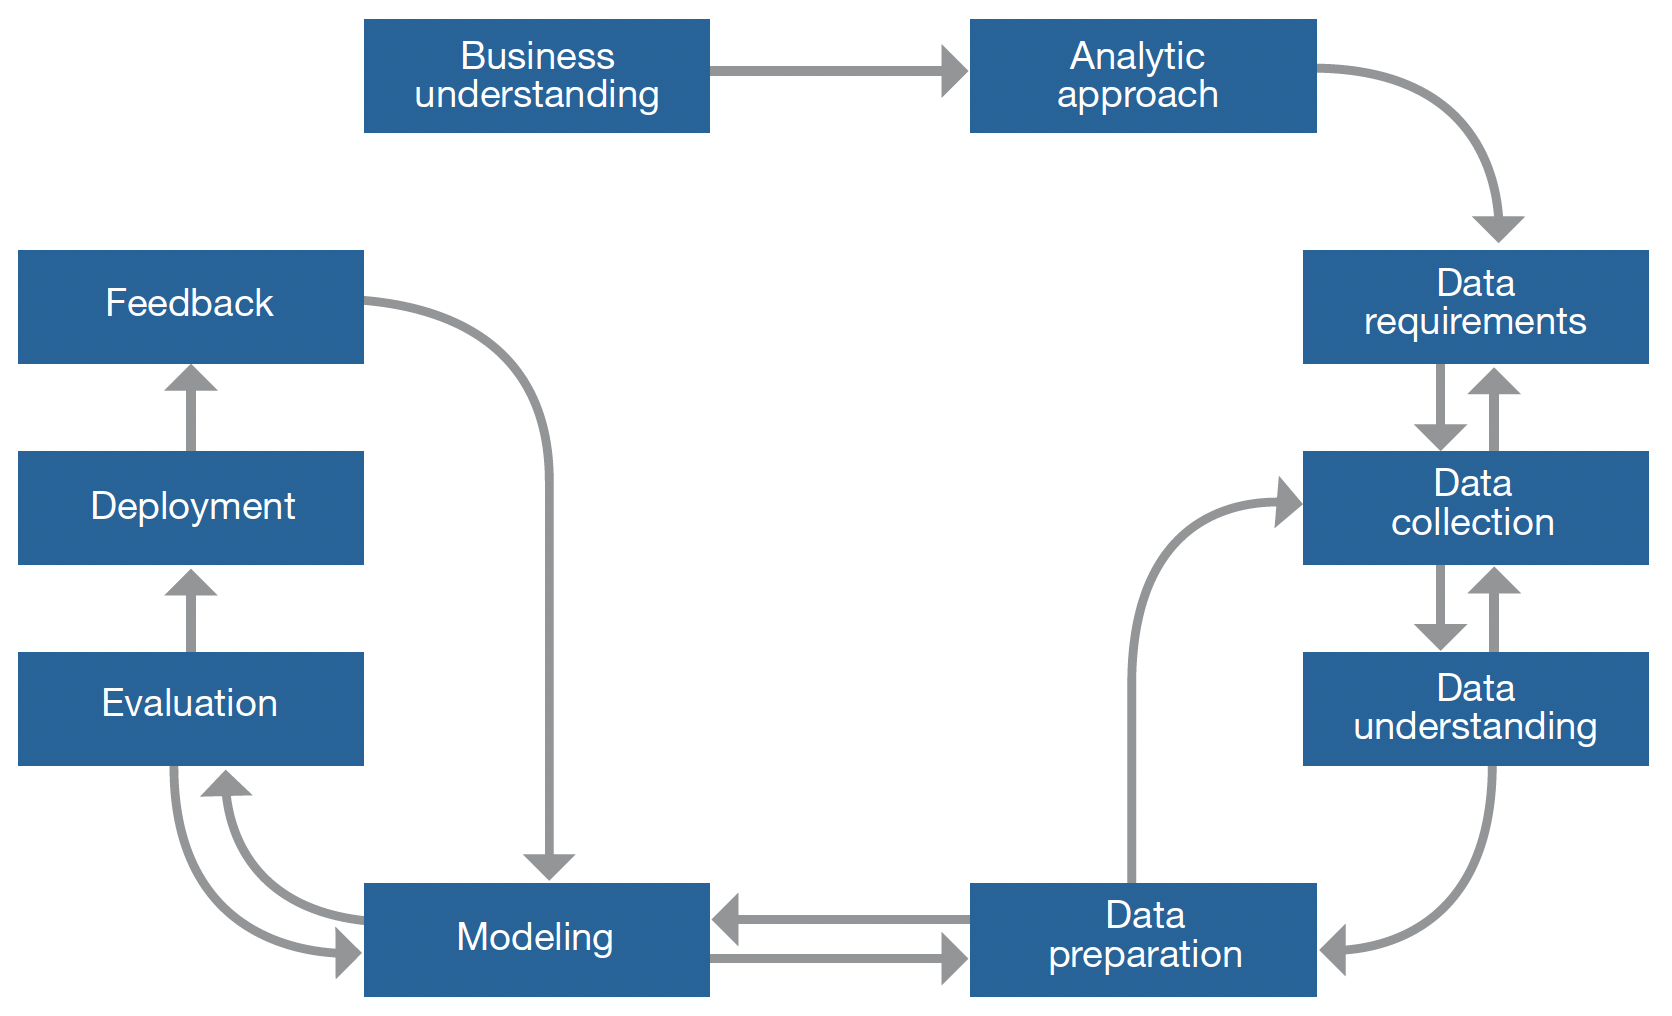
\includegraphics[width=.7\columnwidth]{Imagenes/methodology}
	\caption{Metodología Fundamental para la Ciencia de Datos}
	\label{fig:etapas-metodologia-fundamental}
\end{figure}			
Para llevar a cabo el análisis de datos, se adoptó la \textit{Metodología Fundamental para la Ciencia de Datos}, propuesta por John Rollins en 2015 \cite{Rollins2015}, cuyas etapas principales se ilustran en la Figura \ref{fig:etapas-metodologia-fundamental}.

Esta metodología consta de diez etapas organizadas en un proceso iterativo, cada una con objetivos y actividades específicas, cubriendo desde la comprensión del problema hasta la implementación de soluciones basadas en datos.

Este enfoque es independiente de cualquier tecnología específica, permitiendo flexibilidad en su aplicación según los requerimientos del estudio. 	
	
	
 	\par	A continuación, se detalla la aplicación de esta metodología en el presente estudio.
 
 \subsection{Business understanding}\label{sec:fase1}
 
 Las licitaciones públicas constituyen un proceso fundamental para asegurar la adquisición de bienes, servicios y obras públicas por parte del estado europeo, donde se busca la transparencia y eficiencia en el uso de los recursos públicos. Sin embargo, este proceso se ve dificultado por la complejidad y el gran volumen de datos involucrados, lo que ocasiona retrasos o posibles errores en la toma de decisiones y selección de propuestas. 

 	Optimizar este proceso mediante el uso de modelos analíticos tiene un impacto económico directo, ya que se estima que una mejora del 1~\% en la eficiencia de las contrataciones públicas podría representar un ahorro anual de hasta 20 mil millones de euros.

	El objetivo de esta fase es comprender las necesidades del dominio y traducirlas en objetivos analíticos concretos. En este sentido, se definieron dos metas principales: (i) desarrollar un modelo capaz de predecir la actividad principal de la entidad contratante (\texttt{MAIN\_ACTIVITY}) y (ii) predecir si una licitación será adjudicada a una pyme (\texttt{SME\_WIN}), definida como la variable binaria que indica si al menos un lote del contrato fue ganado por una pequeña o mediana empresa.

	Asimismo, se establecieron indicadores de éxito que permitan evaluar el impacto de la solución: la precisión alcanzada en la clasificación, la reducción del tiempo de análisis y la mejora en la trazabilidad de los resultados obtenidos.

Por esta razón, implementar un sistema de clasificación  
 que combine técnicas de inteligencia artificial explicable  con sistemas de reglas  representa una estrategia viable  para 
 mejorar la gestión de la información. Esta solución permite reducir los tiempos de análisis y aumenta la precisión en la selección de propuestas y, en consecuencia, contribuye a una administración más efectiva y transparente de los recursos públicos destinados a procesos de licitaciones.

 
  \subsection{Analytic approach}\label{sec:fase2}
  
  El enfoque analítico adoptado en este estudio combina técnicas de análisis exploratorio de datos, aprendizaje automático supervisado y filtrado basado en reglas, con el objetivo de construir un modelo robusto para la clasificación de licitaciones públicas.
  

 	El enfoque seleccionado es de tipo \textit{predictivo y explicativo}, centrado en la identificación de patrones que permitan anticipar el tipo de entidad contratante (\texttt{MAIN\_ACTIVITY}) y la probabilidad de adjudicación a pyme (\texttt{SME\_WIN}).

  Para el modelado se emplean algoritmos de clasificación basados en árboles de decisión: \textit{Random Forest} (\textit{RF}) y \textit{Gradient Boosting Classifier} (\textit{GB}). Estos algoritmos fueron seleccionados debido a su gran  capacidad de manejar conjuntos de datos con múltiples características categóricas y numéricas, así como por su interpretabilidad a través de medidas como la importancia de atributos. 
	Además, ambos modelos ofrecen un  equilibrio adecuado entre precisión, escalabilidad y transparencia, aspectos a considerar en el contexto de las contrataciones públicas \cite{friedman2001greedy,breiman2001random}.

  	En comparación con otros enfoques como las \textit{Deep Neural Networks} (DNNs) pueden alcanzar altos niveles de precisión, pero su estructura de ``caja negra'' limita la transparencia y dificulta su adopción en procesos donde es necesaria la trazabilidad \cite{lipton2018mythos}. Asimismo, modelos como \textit{Support Vector Machines} (SVM) presentan problemas de escalabilidad en grandes volúmenes de datos \cite{joachims1998text}, mientras que los \textit{modelos lineales simples} como la \textit{Logistic Regression} (LR) pueden ser demasiado restrictivos para capturar relaciones no lineales complejas que son habituales en las licitaciones públicas.

 	El enfoque analítico, por tanto, prioriza la interpretabilidad y la transparencia sin comprometer el rendimiento predictivo, integrando técnicas de aprendizaje supervisado con métodos de explicación local (LIME) para fortalecer la confianza y la validación humana de las decisiones del modelo.
  
    En cuanto al entorno tecnológico, se utilizan herramientas ampliamente aplicadas en ciencia de datos y aprendizaje automático. Entre ellas, se encuentra  \textit{Python} como lenguaje principal; \textit{Apache Spark} para el manejo eficiente de grandes volúmenes de datos; \textit{Pandas} para la manipulación de datos; \textit{Matplotlib} y \textit{Seaborn} para la visualización gráfica; y \textit{Scikit-learn} para la construcción, entrenamiento y evaluación de modelos. Finalmente, se emplea \textit{LIME} (\textit{Local Interpretable Model-agnostic Explanations}) para la interpretación de los modelos predictivos, lo que facilita la explicación de las decisiones del sistema y aporta transparencia en el contexto de licitaciones públicas.
  

	Los procedimientos de preprocesamiento y balanceo ---mediante \texttt{RandomOverSampler} de \textit{imbalanced-learn}--- se desarrollan en la fase de \textit{Data Preparation}, garantizando la consistencia metodológica de acuerdo con el marco propuesto por Rollins.

  \subsection{Data requirements}\label{sec:fase3}
 

El análisis se sustenta en un conjunto de datos estructurado que recopila información detallada sobre los procedimientos de contratación pública publicados en la plataforma TED. 
Para garantizar su adecuación al objetivo del estudio, se seleccionaron únicamente los registros completos y consistentes, excluyendo aquellos cancelados y los anteriores al año 2015. 
El periodo analizado abarca de 2015 a 2023, lo que permite disponer de una base representativa y actualizada de las licitaciones europeas. 

	La fuente principal de datos corresponde al conjunto \textit{TED CSV Open Data v3.3}, publicado por la Comisión Europea (2020), que compila más de 500.000 registros anuales de avisos de licitación y adjudicación.


El diseño metodológico adopta un enfoque iterativo compuesto por tres fases principales: \textit{Data Collection}, \textit{Data Understanding} y \textit{Data Preparation}. 
Cada fase se ejecuta de manera secuencial, de modo que la salida de una se convierte en la entrada de la siguiente, permitiendo refinar progresivamente la calidad y relevancia de los datos utilizados para el modelado.


\begin{itemize}
	\item Primera iteración: limpieza y consolidación.
	\item Segunda iteración: análisis exploratorio y selección de características
	\item Tercera iteración: normalización y balanceo.
\end{itemize}

\paragraph{Estructura y contenido del conjunto de datos.} 

El conjunto de datos contiene múltiples categorías de información consideradas esenciales para representar las características estructurales y contextuales de las licitaciones:

\begin{itemize}
	\item Información de la entidad contratante (por ejemplo, \texttt{CAE\_TYPE}, \texttt{CAE\_GPA\_ANNEX}).
	\item Detalles del contrato (por ejemplo, \texttt{TYPE\_OF\_CONTRACT}, \texttt{VALUE\_EURO}, \texttt{DURATION}).
	\item Información geográfica y temporal (por ejemplo, \texttt{ISO\_COUNTRY\_CODE}, \linebreak\texttt{YEAR}, \texttt{WIN\_COUNTRY\_CODE}).
	\item Indicadores de participación de pymes, subcontratación y procedimientos de adjudicación.
	\item Códigos CPV (\textit{Common Procurement Vocabulary}) y actividad principal.
\end{itemize}

\paragraph{Criterios de inclusión de los datos.}
%\dorevisar{
	En la fase inicial del procesamiento se aplicaron filtros propios de los objetivos del estudio, con el propósito de garantizar la calidad y relevancia del conjunto de datos. 
Se consideraron únicamente las licitaciones que no habían sido canceladas, cuyo valor no superaba los 500 millones de euros y que presentaban la mejor relación calidad--precio, garantizando así la homogeneidad y pertinencia de los datos analizados.
	Este umbral se estableció para eliminar valores atípicos que representan menos del 0.1~\% de los registros y que podrían distorsionar las relaciones entre las variables cuantitativas.
Esta restricción permite enfocar el estudio en contratos de gran representatividad, evitando sesgos provocados por adjudicaciones extremadamente atípicas en magnitud.


Una vez definidos los requerimientos de datos, se procedió a su recopilación, depuración y transformación durante las etapas de Data Preparation y Modeling.

 
 %%%%%%%%%% Data requirements - END %%%%%%%%%%%%% 
  
\subsection{Primera iteración: limpieza y consolidación de datos  }

\subsection*{\textbf{Data collection}}\label{sec:fase4-iteracion1}

En esta fase se implementó un flujo de trabajo de tipo ETL (\textit{Extract, Transform, Load}) para organizar y preparar los datos provenientes de la plataforma TED. % (\textit{Tenders Electronic Daily}). 
El proceso de extracción consistió en descargar los archivos CSV oficiales publicados por la Comisión Europea y estructurarlos en un entorno de procesamiento distribuido. 
Posteriormente, se verificó la integridad de los registros, eliminando duplicados y asegurando la coherencia entre los archivos de contratos ya adjudicados (\texttt{CAN}) y de futuras contrataciones (\texttt{CFC}). 
La información consolidada se almacenó en un formato optimizado para su análisis posterior mediante \textit{Apache Spark} y \textit{Pandas}, sentando las bases para las fases de comprensión y preparación de los datos.

\paragraph{\textbf{Proceso ETL.}}\label{sec:etl}

El proceso ETL es fundamental para preparar los datos provenientes de diversas fuentes antes de su análisis. 
A continuación, se describen sus tres etapas principales:


\begin{enumerate}
\item \textbf{Extracción:} Los datos se obtienen directamente desde la plataforma TED, cuyos  
archivos en formato CSV están agrupados en dos categorías: 

\begin{description}
        \item[\textbf{CAN} (\textit{Contract Award Notices}):] Archivos que contienen información detallada sobre los contratos que ya han sido adjudicados, incluyendo datos de la entidad contratante, adjudicatario y valor del contrato.

	\item[\textbf{CFC} (\textit{Contract Forecast Notices}):] Archivos que describen las adquisiciones previstas por las administraciones públicas, con información sobre los procedimientos planificados y sus estimaciones de valor.
	
\end{description}

\item \textbf{Transformación:}  
Se aplican procedimientos de limpieza, conversión y estructuración para garantizar la calidad de los datos. 
%\dorevisar{
Las variables numéricas se verifican y convierten al formato adecuado, mientras que las categóricas se estandarizan en nomenclatura y codificación. 
La normalización y codificación avanzada se desarrollan en la fase posterior de \textit{Data Preparation}.
%}

\item \textbf{Carga:} Los datos procesados se almacenan en una estructura optimizada para su análisis posterior. En este proyecto, los datos se cargan inicialmente en \textit{Apache Spark} debido a su eficiencia en el manejo de grandes volúmenes de datos y, posteriormente, se convierten a \textit{Pandas} para facilitar el análisis exploratorio y la visualización de resultados.

\end{enumerate}

\noindent Esta fase permitió consolidar un conjunto de datos estructurado, consistente y actualizado, que sirve de base para las etapas de comprensión y preparación descritas a continuación.


%%%%%%%%%% Data collection - END %%%%%%%%%%%%% 

\subsection*{Data understanding}\label{sec:fase5-iteracion1}

En esta fase se busca comprender la estructura, coherencia y relaciones internas del conjunto de datos recopilado. 
Los archivos CAN y CFC, aunque comparten ciertas características, representan etapas distintas del proceso de contratación: 
los primeros contienen información sobre contratos adjudicados, mientras que los segundos recogen las adquisiciones previstas.

La unificación de ambos conjuntos de datos permitió generar un registro consolidado de todos los contratos efectivamente adjudicados, 
descartando aquellos que aún no han sido asignados, a pesar de que deberían contar con una adjudicación\footnote{Es importante aclarar que este proceso no implica una evaluación ética de las licitaciones, sino una depuración técnica basada en la información disponible en los repositorios de TED. Por lo que, el análisis de los datos se centra únicamente en su coherencia y estructura, sin realizar ningún tipo de interpretación a las normas ni regulaciones.}. 
%
Estos registros podrían introducir ruido en el modelo de ML en desarrollo, afectando su rendimiento al generar inconsistencias en los datos de entrenamiento.

La relación entre estos dos conjuntos de datos está definida a través de las características \texttt{ID\_NOTICE\_CAN} (presente en los archivos CAN) y \texttt{FUTURE\_CAN\_ID}, utilizada en los archivos CFC. Esta vinculación permite realizar un  cruce  de datos de manera consistente para su posterior análisis.

\paragraph{\textbf{Análisis exploratorio.}}

%\dorevisar{
	Posteriormente, se realizó un análisis univariable y bivariable para comprender la distribución, correlación y posibles valores atípicos entre las características más relevantes del conjunto de datos. Este análisis sirve como base para la selección de las características clave que se incorporarán al modelo de clasificación.
%	}

La Tabla \ref{tab:variables} presenta las características resultantes de la unificación de ambos archivos, conformando un conjunto de 96 características con un total de aproximadamente 340.46 millones de datos en bruto. Cada una de estas características desempeña un papel específico dentro del análisis. %, facilitando la estructuración y posterior procesamiento del modelo.

%\begin{table}[htb]	
%\begin{table}[HT]	
\begin{table*}[t]
	\centering
	\scriptsize
%	\small
	  \setlength{\tabcolsep}{7pt} 
	\renewcommand{\arraystretch}{1.3} % Aumenta el espacio entre filas
	\caption{Características del conjunto de datos} \label{tab:variables} 	
	\begin{adjustbox}{max width=\textwidth}	
		\begin{tabular}{p{4cm}p{4.2cm}p{4.7cm}}		
			\hline
			\multicolumn{3}{c}{\textsc{\textbf{Características}}} \\ \hline
	
	% Características ordenadas alfabéticamente
	\texttt{ADDITIONAL\_CPVS} & \texttt{ADMIN\_LANGUAGE\_TENDER} & \texttt{ADMIN\_OTHER\_LANGUAGES\_TENDER} \\
	\texttt{AWARD\_EST\_VALUE\_EURO} & \texttt{AWARD\_VALUE\_EURO} & \texttt{AWARD\_VALUE\_EURO\_FIN\_1} \\
	\texttt{B\_ACCELERATED} & \texttt{B\_AWARDED\_BY\_CENTRAL\_BODY} & \texttt{B\_AWARDED\_TO\_A\_GROUP} \\
	\texttt{B\_CONTRACTOR\_SME} & \texttt{B\_DYN\_PURCH\_SYST} & \texttt{B\_ELECTRONIC\_AUCTION} \\
	\texttt{B\_EU\_FUNDS} & \texttt{B\_FRA\_AGREEMENT} & \texttt{B\_FRA\_CONTRACT} \\
	\texttt{B\_FRA\_SINGLE\_OPERATOR} & \texttt{B\_GPA} & \texttt{B\_INVOLVES\_JOINT\_PROCUREMENT} \\
	\texttt{B\_LANGUAGES\_ANY\_EC} & \texttt{B\_MULTIPLE\_CAE} & \texttt{B\_MULTIPLE\_COUNTRY} \\
	\texttt{B\_ON\_BEHALF} & \texttt{B\_OPTIONS} & \texttt{B\_RECURRENT\_PROCUREMENT} \\
	\texttt{B\_RENEWALS} & \texttt{B\_SUBCONTRACTED} & \texttt{B\_VARIANTS} \\
	\texttt{CAE\_ADDRESS} & \texttt{CAE\_GPA\_ANNEX} & \texttt{CAE\_NAME} \\
	\texttt{CAE\_NATIONAL\_ID} & \texttt{CAE\_POSTAL\_CODE} & \texttt{CAE\_TOWN} \\
	\texttt{CAE\_TYPE} & \texttt{CANCELLED} & \texttt{CONTRACT\_COMPLETION} \\
	\texttt{CONTRACT\_NUMBER} & \texttt{CONTRACT\_START} & \texttt{CORRECTIONS} \\
	\texttt{CPV} & \texttt{CRIT\_CODE} & \texttt{CRIT\_CRITERIA} \\
	\texttt{CRIT\_PRICE\_WEIGHT} & \texttt{CRIT\_WEIGHTS} & \texttt{DT\_APPLICATIONS} \\
	\texttt{DT\_AWARD} & \texttt{DT\_DISPATCH} & \texttt{DURATION} \\
	\texttt{ENV\_MAX\_OPERATORS} & \texttt{ENV\_MIN\_OPERATORS} & \texttt{ENV\_OPERATOS} \\
	\texttt{EU\_INST\_CODE} & \texttt{FRA\_ESTIMATED} & \texttt{FRA\_NUMBER\_MAX\_OPERATOS} \\
	\texttt{FRA\_NUMBER\_OPERATORS} & \texttt{FUTURE\_CAN\_ID} & \texttt{FUTURE\_CAN\_ID\_ESTIMATED} \\
	\texttt{GPA\_COVERAGE} & \texttt{ID\_AWARD} & \texttt{ID\_LOT} \\
	\texttt{ID\_LOT\_AWARDED} & \texttt{ID\_NOTICE\_CAN} & \texttt{ID\_NOTICE\_CN} \\
	\texttt{ID\_TYPE} & \texttt{INFO\_ON\_NON\_AWARD} & \texttt{INFO\_UNPUBLISHED} \\
	\texttt{ISO\_COUNTRY\_CODE} & \texttt{ISO\_COUNTRY\_CODE\_ALL} & \texttt{ISO\_COUNTRY\_CODE\_GPA} \\
	\texttt{LOTS\_NUMBER} & \texttt{LOTS\_SUBMISSION} & \texttt{MAIN\_ACTIVITY} \\
	\texttt{MAIN\_CPV\_CODE\_GPA} & \texttt{NUMBER\_AWARDS} & \texttt{NUMBER\_OFFERS} \\
	\texttt{NUMBER\_OFFERS\_ELECTR} & \texttt{NUMBER\_TENDERS\_NON\_EU} & \texttt{NUMBER\_TENDERS\_OTHER\_EU} \\
	\texttt{NUMBER\_TENDERS\_SME} & \texttt{OUT\_OF\_DIRECTIVES} & \texttt{TAL\_LOCATION\_NUTS} \\
	\texttt{TED\_NOTICE\_URL} & \texttt{TITLE} & \texttt{TOP\_TYPE} \\
	\texttt{TYPE\_OF\_CONTRACT} & \texttt{VALUE\_EURO} & \texttt{VALUE\_EURO\_FIN\_1} \\
	\texttt{VALUE\_EURO\_FIN\_2} & \texttt{WIN\_ADDRESS} & \texttt{WIN\_COUNTRY\_CODE} \\
	\texttt{WIN\_NAME} & \texttt{WIN\_NATIONALID} & \texttt{WIN\_POSTAL\_CODE} \\
	\texttt{WIN\_TOWN} & \texttt{XSD\_VERSION} & \texttt{YEAR} \\
	\hline
	
	\end{tabular}
\end{adjustbox}		


\end{table*}	
    
    
%%%%%%%%%% Data understanding - END %%%%%%%%%%%%%    

\subsection*{Data preparation}\label{sec:fase6-iteracion1}



\noindent\textbf{\textit{Eliminación de columnas.}}
Se eliminaron aquellas características irrelevantes o redundantes que no aportaban información significativa al estudio. 
Esto incluye variables con valores repetitivos o de baja variabilidad, así como aquellas con registros insuficientes para ser estadísticamente representativos. 
La Tabla~\ref{tab:variables-candidatas1} presenta el conjunto inicial de 25 características candidatas seleccionadas por su relevancia en el rendimiento del modelo.



\begin{table*}[t]
	\centering
	\scriptsize
%	\small
	  \setlength{\tabcolsep}{7pt} 
	\renewcommand{\arraystretch}{1.3} % Aumenta el espacio entre filas
	\caption{Conjunto inicial de {características candidatas}} 
	\label{tab:variables-candidatas1} 	
	\begin{adjustbox}{max width=\textwidth}
		\begin{tabular}{ll}
			\hline

	\multicolumn{1}{c}{\textbf{\textsc{Característica}}} & \multicolumn{1}{c}{\textbf{\textsc{Descripción}}}  \\
	\hline
	
	% Características ordenadas alfabéticamente
	\texttt{B\_CONTRACTOR\_SME}    & Indica si es pyme. \\	
%	\texttt{B\_MULTIPLE\_CAE}      & Indica las CAE (\textit{Contracting Authority Entity})\footnotemark{} asociadas \\
	\texttt{B\_MULTIPLE\_CAE}      & Indica las CAE (\textit{Contracting Authority Entity}) asociadas.\\
	%	\texttt{B\_ON\_BEHALF}         & Indica si se realizó desde otra entidad \\
	\texttt{B\_ON\_BEHALF}         & Indica si es una compra conjunta.  \\	
	\texttt{B\_SUBCONTRACTED}      & Indica si fue contratado. \\
%	\texttt{CAE\_GPA\_ANNEX}       & CAE asociada al GPA\footnotemark{}. \\
\texttt{CAE\_GPA\_ANNEX}       & CAE asociada al GPA (\textit{Government Procurement Agreement}). \\
	\texttt{CAE\_NAME}             & Entidad asociada a la CAE. \\
	\texttt{CAE\_TOWN}             & Ciudad asociada a la CAE. \\
	\texttt{CAE\_TYPE}             & Tipo de autoridad contratante. \\
%	\texttt{CANCELLED*}                       & Indica si fue cancelado \\
	\texttt{CPV}                             & Clasificación del producto. \\
	\texttt{CRIT\_CODE}            & Indica el código de criterio. \\
	\texttt{CRIT\_CRITERIA}        & Criterios a tener en cuenta de la licitación. \\
	\texttt{CRIT\_PRICE\_WEIGHT}   & Precio en base al criterio. \\
	\texttt{CRIT\_WEIGHTS}         & Criterios de los pesos. \\
	\texttt{DURATION}              & Duración del contrato. \\
	\texttt{ID\_TYPE}              & Tipo de Identificador. \\
%	\texttt{ISO\_COUNTRY\_CODE}    & Código ISO\footnotemark{} del País. \\
\texttt{ISO\_COUNTRY\_CODE}    & Código ISO (\textit{International Organization for Standardization}) del País. \\
	\texttt{LOTS\_NUMBER}          & Número de lotes para una convocatoria de concurso específica.\\
	\texttt{MAIN\_ACTIVITY}        & Actividad Principal. \\
	\texttt{NUMBER\_AWARDS}        & Número de contratos otorgados. \\
	\texttt{NUMBER\_OFFERS}        & Número de licitaciones. \\
	\texttt{NUMBER\_TENDERS\_SME}  & Número de pyme. \\
	\texttt{TOP\_TYPE}             & Tipo de procedimiento de la licitación.\\
	\texttt{TYPE\_OF\_CONTRACT}    & Tipo de contrato. \\
	\texttt{VALUE\_EURO}           & Valor del euro. \\
	\texttt{WIN\_COUNTRY\_CODE}    & Código del país ganador.\\
%	\texttt{YEAR*}                            & Año \\	
	\hline
	
	\end{tabular}
\end{adjustbox}	
%\vspace{1ex}

\end{table*}

\noindent\textbf{\textit{Filtrado de datos.}}
%
Para asegurar  la calidad de los datos, es necesario eliminar aquellos registros %irrelevantes 
que no cumplen con los criterios de selección establecidos,
ya que su inclusión no aporta información relevante al modelo.  
Estos criterios de selección se detallan en la Tabla \ref{tab:condiciones}. 

Entre estos criterios, se descartan  los registros cuya característica \texttt{CRIT\_CODE} sea diferente de ``M'', 
ya que representan un subconjunto mínimo de datos sin impacto significativo en el modelo. En este contexto, ``M'' hace referencia a la oferta económicamente más ventajosa, la cual prioriza la mejor relación calidad--precio en lugar de únicamente el menor costo, que es el enfoque de este estudio. 


\begin{table*}[t]
	\centering
	\scriptsize
%	\small
  \setlength{\tabcolsep}{7pt} 
	\renewcommand{\arraystretch}{1.3} % Aumenta el espacio entre filas
	\caption{Condiciones para la eliminación de datos.}		
\begin{adjustbox}{max width=\textwidth}
	\begin{tabular}{p{3.5cm}p{9cm}}
		\hline
		\multicolumn{1}{c}{\textbf{\textsc{Variable}}} & \multicolumn{1}{c}{\textbf{\textsc{Condición}}} \\ 
		\hline
		\texttt{CANCELLED} & Contratos que no han sido cancelados. \\ 
		\texttt{CRIT\_CODE} & Tipo de criterio sólo ``M''. \\ 
		\texttt{CRIT\_PRICE\_WEIGHT} & Pesos del precio mayores a 0. \\ 
		\texttt{DURATION} & Duración de contratos que son mayores a 0.  \\ 
		\texttt{LOTS\_NUMBER} & Número de lotes mayores a 1. \\ 
		\texttt{NUMBER\_AWARDS} & Número de contratos otorgados menores o iguales a 0. \\ 
		\texttt{NUMBER\_OFFERS} & Número de licitantes presentados menores o iguales a 0.  \\ 
		\texttt{NUMBER\_TENDERS\_SME} & Número de licitantes de pequeñas y medianas empresas mayores a 0. \\ 
		\texttt{TOP\_TYPE} & Tipo de procedimiento diferente de AWP y NOC/NOP. \\ 
		\texttt{VALUE\_EURO} & Costos totales de los contratos mayor o igual a 1.000 y menor o igual a 50 millones de euros. \\ 
		\hline
	\end{tabular}
\end{adjustbox}	
%	\vspace{1ex}
	\label{tab:condiciones}
\end{table*}



%\noindent\textbf{\textit{Conversión a minúsculas.}}
\paragraph{\textbf{Estandarización de texto y codificación.}}

Para mantener la uniformidad en los datos y evitar los sesgos en la clasificación, es necesario estandarizar el formato de las palabras, ya que algunas pueden aparecer en mayúsculas, minúsculas o con una combinación de ambas; se realiza la conversión de todos los textos a minúsculas. 

\paragraph{\textbf{Normalización y codificación de variables.}}

%\dorevisar{
	Las variables numéricas se normalizan, mientras que las variables categóricas se codifican mediante la técnica  \textit{OneHotEncoder}\footnote{El \textit{OneHotEncoder} convierte las categorías en variables binarias independientes, facilitando su uso en modelos de aprendizaje automático. Por ejemplo, una variable \textit{Color} con categorías \textit{Rojo}, \textit{Verde} y \textit{Azul} se transformaría en tres columnas binarias: \textit{Color\_Rojo}, \textit{Color\_Verde} y \textit{Color\_Azul}.}.
	%
	Esta técnica es ampliamente recomendada, ya que evita que el modelo interprete relaciones ordinales inexistentes entre categorías, preservando la independencia semántica entre las clases y reduciendo sesgos en el aprendizaje \cite{geron2019hands}. Además,  permite representar cada categoría como una dimensión separada dentro del espacio de características, lo que mejora la interpretabilidad del modelo y asegura que las distancias o criterios de división sean coherentes \cite{raschka2020python}. Es conjunto, esta forma de codificación proporciona un preprocesamiento más estable, reproducible y adecuado para el entrenamiento de modelos de clasificación supervisada.
%	}

\paragraph{\textbf{Tratamiento de valores faltantes y duplicados.}}

Las variables numéricas con baja desviación estándar fueron imputadas con sus valores mínimos, mientras que las categóricas se completaron con la moda, seleccionando el valor más frecuente dentro de cada característica.  
Finalmente, se eliminaron los registros duplicados para asegurar la integridad del conjunto.



\par\vspace{1em}\noindent Después de aplicar el proceso de depuración y consolidación, el número de registros resultantes es de 
159,752 y  25 características candidatas, mostradas en la Tabla \ref{tab:variables-candidatas1}.


%%%%%%%%%%%%%%%%%%%% FIN PRIMERA ITERACIÓN %%%%%%%%%%%%%



\subsection{Segunda iteración: análisis exploratorio y selección de características}

%\noindent
Esta fase tiene como propósito realizar el análisis exploratorio y la selección de características del conjunto de datos, con el fin de identificar aquellas variables que aportan información significativa al modelo y eliminar las redundantes o irrelevantes. 
%Se estructura en tres etapas: \textit{Data Collection}, \textit{Data Understanding} y \textit{Data Preparation}.


\subsection*{Data collection}

Algunas características numéricas pueden agruparse en rangos, como ``\texttt{DURATION}'' y \linebreak``\texttt{VALUE\_EURO}''. Para determinar el número óptimo de clases, se aplicó la \textit{regla de Sturges}, que establece el número de intervalos en función del tamaño del conjunto de datos. La fórmula utilizada es:

\begin{equation}
	k = 1 + 3.322 \log_{10}(n)
\end{equation}

Por otro lado, la variable \texttt{CPV} se agrupó a partir de los dos primeros dígitos de su código, creando la columna \texttt{GROUP\_CPV}, la cual permite representar de forma agregada las categorías principales de actividad económica.


\subsection*{Data understanding}

En esta fase se realiza un análisis univariable de las características candidatas, diferenciando entre variables numéricas y categóricas, con el objetivo de comprender su distribución, variabilidad y posible sesgo.

La Tabla~\ref{tab:variables-numericas} muestra las estadísticas descriptivas de las variables numéricas, incluyendo medidas de tendencia central y dispersión. 
Se observan distribuciones asimétricas en variables como \texttt{VALUE\_EURO} y \texttt{LOTS\_NUMBER}, donde la diferencia entre la media y la mediana evidencia la presencia de valores extremos.


\begin{table*}[t]
%	\scriptsize
	\small
	\centering
	\setlength{\tabcolsep}{4pt}
	\renewcommand{\arraystretch}{1.3} % Aumenta el espacio entre filas
	\caption{Estadísticas Descriptivas de las variables numéricas}
	\label{tab:variables-numericas}		
	\begin{adjustbox}{max width=\textwidth}
		\begin{tabular}{lrrrrrrr} 
%			\begin{tabular}{p{3.2cm} *{7}{m{1.7cm}}} 
			\hline
			\multicolumn{1}{c}{\textbf{\textsc{Características}}} & 
			\multicolumn{1}{c}{\textbf{\textsc{Mínimo}}} & 
			\multicolumn{1}{c}{\textbf{\textsc{Máximo}}} & 
			\multicolumn{1}{c}{\textbf{\textsc{Media}}} & 
%			\textbf{Desviación estándar} & 
			\multicolumn{1}{c}{\shortstack{\textbf{\textsc{Desviación}} \\ \textbf{\textsc{estándar}}}} &			
			\multicolumn{1}{c}{\hspace{0.3cm}\textbf{\textsc{Q1}}\hspace{0.3cm}} & 
			\multicolumn{1}{c}{\shortstack{\textbf{\textsc{Q2}} \\ \textbf{(\textsc{Mediana})}}} & 
			\multicolumn{1}{c}{\hspace{0.3cm}\textbf{\textsc{Q3}} \hspace{0.3cm}} \\
			\hline
			\texttt{CRIT\_PRICE\_WEIGHT} & 1.00 & 1,948,410.00 & 107.38 & 6,722.67 & 60.0 & 60.00 & 80.0 \\ 			
%			\texttt{CRIT\_PRICE\_WEIGHT} & 1.00 & 1.95 M & 107.38 & 6.72 k & 60.00 & 60.00 & 80.00 \\ 			
			\texttt{DURATION} & 1.00 & 1,200.00 & 27.30 & 27.56 & 9.00 & 15.00 & 24.67 \\ 
			\texttt{LOTS\_NUMBER} & 2.00 & 757.00 & 18.15 & 35.83 & 3.00 & 7.00 & 17.00 \\ 
			\texttt{NUMBER\_AWARDS} & 1.00 & 1,065.00 & 21.45 & 45.82 & 4.00 & 8.00 & 20.00 \\ 
			\texttt{NUMBER\_OFFERS} & 1.00 & 321.00 & 3.72 & 5.96 & 1.00 & 3.00 & 4.00 \\ 
			\texttt{NUMBER\_TENDERS\_SME} & 1.00 & 311.00 & 2.96 & 4.21 & 1.00 & 2.00 & 3.00 \\ 
\texttt{VALUE\_EURO} & 1,001.00 & 50,000,000.00 & 2,518,638.80 & 6,010,806.31 & 225,888.00 & 548,437.00 & 1,680,165.75 \\ 
%			\texttt{VALUE\_EURO} & 1.00 k & 50 M & 2.52 M & 6.01 M & 225 k & 548 k & 1.68 M\euro \\ 			
			\hline
		\end{tabular}
	\end{adjustbox}
%	\vspace{1ex}	

\end{table*}

La Tabla~\ref{tab:variables-categoricas} presenta los resultados para las variables categóricas. 
El número de valores únicos (\textit{Único}) y la frecuencia del modo (\textit{Más común}) permiten detectar variables de alta cardinalidad, como \texttt{CAE\_NAME} o \texttt{CPV}, que contienen miles de valores distintos. 
Esta observación motiva la necesidad de aplicar técnicas de codificación para su posterior uso en los modelos de aprendizaje automático.

\begin{table*}[t]
	\scriptsize
%	\small
	\centering
	\setlength{\tabcolsep}{7pt}
	\renewcommand{\arraystretch}{1.3} % Aumenta el espacio entre filas
	\caption{Estadísticas Descriptivas de las variables categóricas}
	\label{tab:variables-categoricas}		
	\begin{adjustbox}{max width=\textwidth}
		\begin{tabular}{lrcr} % SIN barras "|"
%			\begin{tabular}{p{3.5cm} m{3cm} m{5cm} p{3cm} } 			
			\hline
			\multicolumn{1}{c}{\textbf{\textsc{Características}}} & 
			\multicolumn{1}{c}{\textbf{\textsc{Único}}} & 
			\multicolumn{1}{c}{\textbf{\textsc{Más común}}} & 
			\multicolumn{1}{c}{\shortstack{\textbf{\textsc{Frecuencia}} \\ \textbf{\textsc{absoluta}}}}  \\
			\hline
			\texttt{B\_CONTRACTOR\_SME} & 630 & y & 110,193 \\%\hline
			\texttt{B\_MULTIPLE\_CAE} & 2 & N & 154,160 \\%\hline
			\texttt{B\_ON\_BEHALF} & 2 & N & 147,980 \\%\hline
			\texttt{B\_SUBCONTRACTED} & 2 & N & 147,308 \\ %\hline
			\texttt{CAE\_GPA\_ANNEX} & 2 & N & 154,160 \\ %\hline
			\texttt{CAE\_NAME} & 14,559 & pa?stwowe gospodarstwo wodne wody polskie & 1,711 \\ %\hline
			\texttt{CAE\_TOWN} & 6,114 & warszawa & 10,601 \\ %\hline
			\texttt{CAE\_TYPE} & 9 & 8 & 54,860 \\ %\hline
			\texttt{CPV} & 3,341 & 33,100,000 & 8,673 \\ %\hline
			\texttt{CRIT\_CRITERIA} & 32,478 & termin dostawy & 6,424 \\ %\hline
			\texttt{CRIT\_WEIGHTS} & 4,840 & 40 & 36,050 \\ %\hline
			\texttt{ID\_TYPE} & 2 & 3 & 153,436 \\ %\hline
			\texttt{ISO\_COUNTRY\_CODE} & 30 & PL & 63,038 \\ %\hline
			\texttt{MAIN\_ACTIVITY} & 21 & health & 50,218 \\ %\hline
			\texttt{TOP\_TYPE} & 6 & OPE & 155,070 \\ %\hline
			\texttt{TYPE\_OF\_CONTRACT} & 3 & U & 99,506 \\ %\hline
			\texttt{WIN\_COUNTRY\_CODE} & 677 & pl & 56,390 \\ %\hline
			\texttt{YEAR} & 9 & 2,023 & 28,916 \\\hline
		\end{tabular}
	\end{adjustbox}
%	\vspace{1ex}		

\end{table*}

\subsection*{Data preparation}

\paragraph{\textbf{Transformación de variables categóricas.}  }

Las variables categóricas no pueden compararse de forma directa en modelos numéricos, por lo que se aplicó la técnica de \textit{OneHotEncoder}, que transforma cada valor único en una nueva variable binaria. 
%
Esta transformación facilita la identificación de relaciones entre las categorías originales y otras variables del conjunto de datos \cite{AdrianRocha}.

Por ejemplo, la variable \texttt{TOP\_TYPE}, con seis categorías, genera seis columnas binarias después de la transformación. 
La Figura~\ref{fig:onehot-toptype} ilustra este proceso: el eje Y de la subfigura (a) representa los valores originales, mientras que (b) muestra las columnas binarias resultantes.

\begin{figure*}[t]
	\caption[Aplicación de OneHotEncoder sobre la variable categórica \texttt{TOP\_TYPE}]{Aplicación de \textit{OneHotEncoder} sobre la variable categórica \texttt{TOP\_TYPE}}
%\label{fig:datos-variables-categoricas}	
\label{fig:onehot-toptype}
	\centering	
	\begin{minipage}{0.42\textwidth} % 48% del ancho de la página
		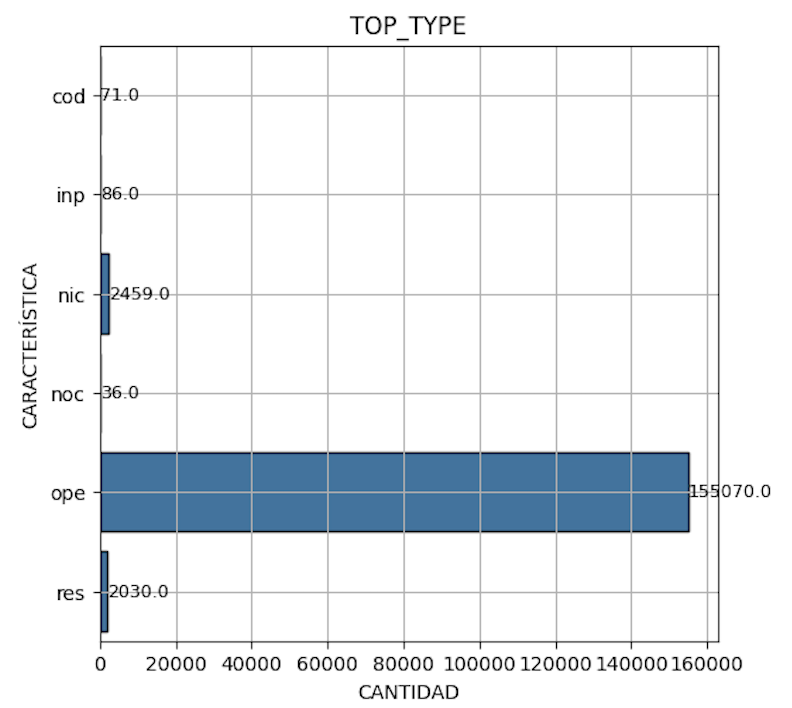
\includegraphics[width=1\textwidth]{Imagenes/fig-010}		
		\centering\textit{(a)}
	\end{minipage}%
%	\hfill
	\begin{minipage}{0.57\textwidth} % 48% del ancho de la página
		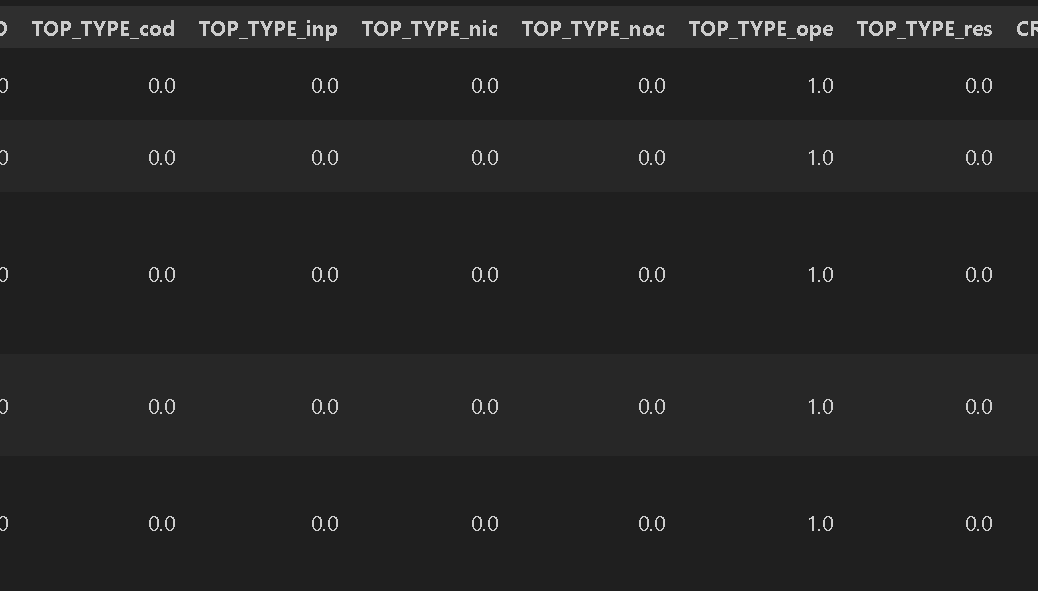
\includegraphics[width=1\textwidth]{Imagenes/oneHotEncoder.png}
		\centering\textit{(b)}		
	\end{minipage}

\end{figure*}


\paragraph{\textbf{Análisis de correlación y selección de variables.}}   

Una vez transformadas las variables categóricas, se evaluaron las relaciones entre variables mediante una matriz de correlación de Pearson, seleccionando aquellas con una correlación absoluta mayor o igual a 0.5. 
Este umbral indica una asociación moderada o fuerte y permite identificar relaciones lineales relevantes para el modelo.
En este contexto, la correlación de Pearson es una de las métricas más utilizadas para medir la relación lineal entre dos variables \cite{james2021isl,kuhn2013applied}.

Si dos variables presentan una correlación de 1, una de ellas se descarta para evitar redundancia \cite{Lalinde2018}.
La Figura \ref{fig:correlacion} muestra las características seleccionadas para el diseño del modelo de ML aplicando este criterio. 

\begin{figure*}[t]
%\begin{figure}[H]
	\caption{Variables seleccionadas}
	\label{fig:correlacion}	
	\centering
	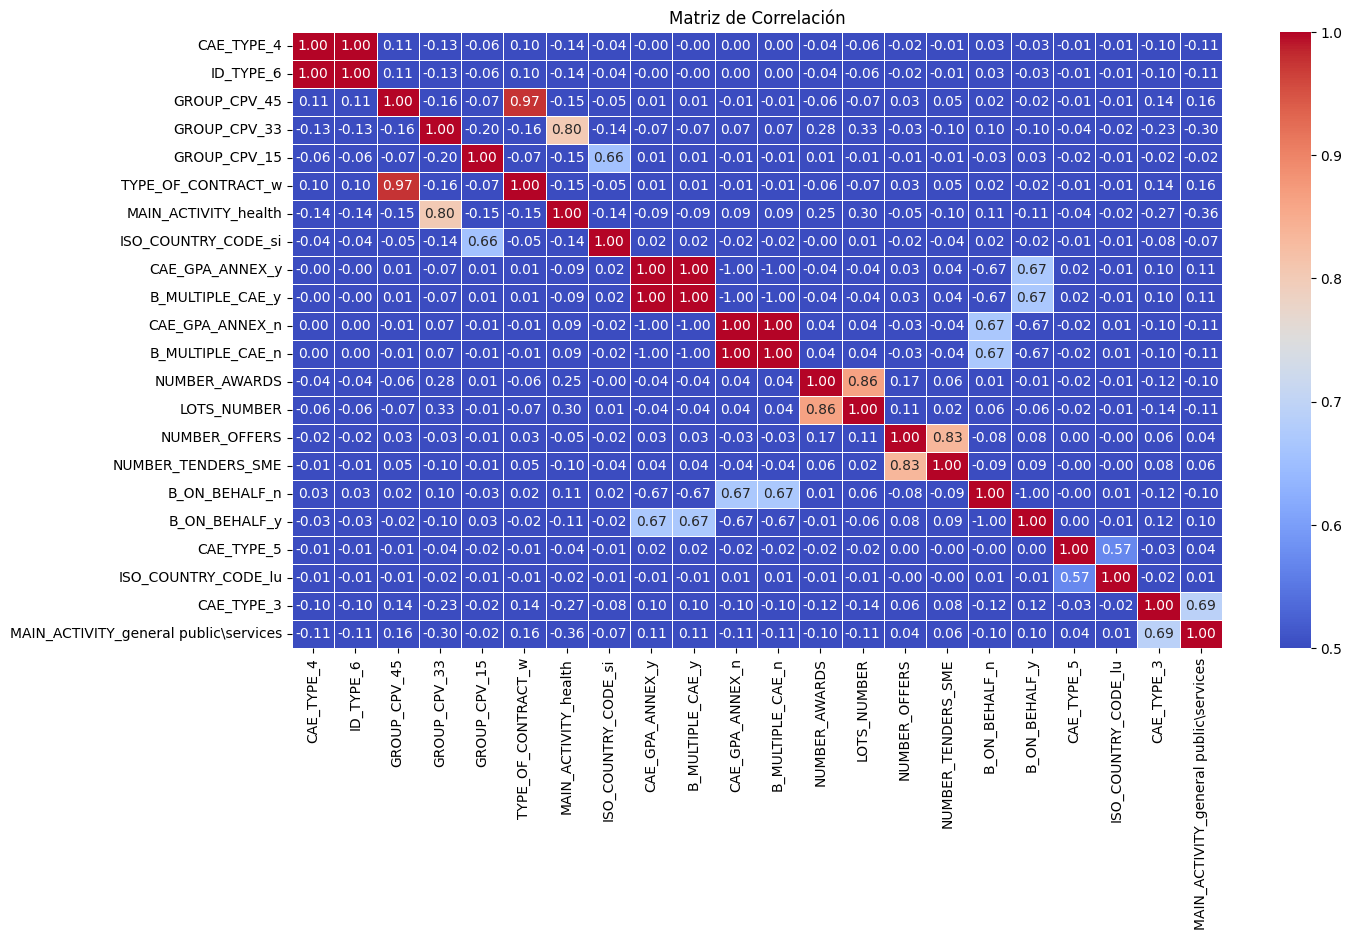
\includegraphics[width=1\textwidth]{Imagenes/bivariable/correlacion_variable_numerica_categorica_2.png}
	%		\vspace{1ex}
	
\end{figure*}

La Figura~\ref{fig:correlacion-bivariable} ilustra dos ejemplos: 
en (a), la relación entre \texttt{CAE\_GPA\_ANNEX\_n} (eje X)  y \texttt{B\_ON\_BEHALF\_n}  (eje Y) muestra una asociación fuerte, mientras que en (b), la relación entre \texttt{LOTS\_NUMBER} y \texttt{NUMBER\_AWARDS} refleja una tendencia positiva, indicando que el número de lotes licitados influye en la cantidad de contratos adjudicados.

\begin{figure*}[t]
%\begin{figure}[H]
	\caption{Análisis exploratorio bivariable entre }
	\label{fig:correlacion-bivariable}	
	\centering	
	\begin{minipage}{0.49\textwidth} % 48% del ancho de la página
		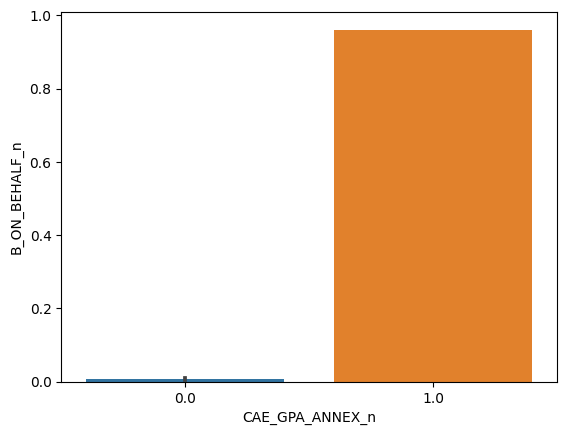
\includegraphics[width=1\textwidth]{Imagenes/bivariable/analisis_relacion_uno}		
		\centering\textit{(a)}
	\end{minipage}%
	\hfill
	\begin{minipage}{0.49\textwidth} % 48% del ancho de la página
		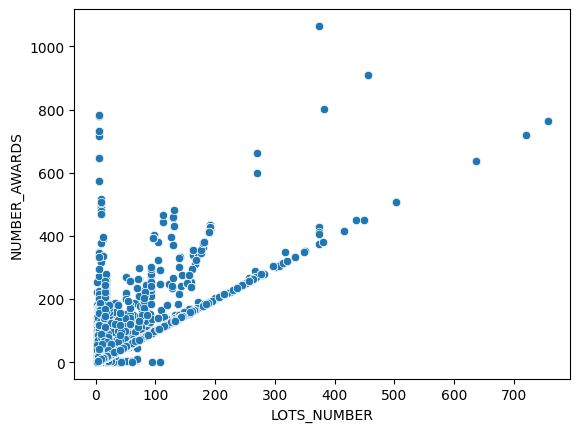
\includegraphics[width=1\textwidth]{Imagenes/bivariable/analisis_relacion_siete}
		\centering\textit{(b)}		
	\end{minipage}	
	
\end{figure*}

Cabe señalar que los valores asociados a las variables \texttt{LOTS\_NUMBER} y \texttt{NUMBER\_AWARDS} pueden variar según los requerimientos específicos de cada licitación. 
De igual modo, el número de ofertas (\texttt{NUMBER\_OFFERS}) depende directamente del número de licitantes o adjudicatarios potenciales.

Las variables seleccionadas tras este análisis se presentan en la Tabla~\ref{tab:variables-seleccionadas}, que resume tanto las variables binarias resultantes del proceso de codificación como las cuantitativas originales. 


\begin{table*}[t]
		\scriptsize
%	\small
	\setlength{\tabcolsep}{7pt}
	\renewcommand{\arraystretch}{1.3} % Aumenta el espacio entre filas
	\caption{Características seleccionadas}
	\label{tab:variables-seleccionadas} 
	\begin{adjustbox}{max width=\textwidth}	
		%		\begin{tabular}{|p{3.5cm}|p{5.75cm}|l|l|}		
			\begin{tabular}{p{3.5cm}p{5.75cm}ll}					
				\hline
				\multicolumn{1}{c}{\textbf{\textsc{Características}}} &
				\multicolumn{1}{c}{\textbf{\textsc{Descripción}}}  &
				\multicolumn{1}{c}{\shortstack{\textbf{\textsc{Valores}} \\ \textbf{\textsc{fijos}}}} &
				\multicolumn{1}{c}{\shortstack{\textbf{\textsc{Valores}} \\ \textbf{\textsc{variables}}}} \\ 
				\hline
				\texttt{B\_MULTIPLE\_CAE\_n}      & No hay múltiples autoridades contratantes                         & 1 = Sí, 0 = No              &                            \\ %\hline
				\texttt{B\_ON\_BEHALF\_n}         & No se realiza desde otra entidad                                  & 1 = Sí, 0 = No              &                            \\ %\hline
				\texttt{CAE\_TYPE\_3}             & Tipo de autoridad contratante  ``Regional or local authority''     & 1 = Sí, 0 = No          &                            \\ %\hline
				\texttt{CAE\_TYPE\_4}             & Tipo de autoridad contratante ``Water, energy, transport and telecommunications sectors'' & 1 = Sí, 0 = No &  \\ %\hline
				\texttt{CAE\_TYPE\_5}             & Tipo de autoridad contratante ``European Union institution/agency'' & 1 = Sí, 0 = No          &                            \\ %\hline
				\texttt{GROUP\_CPV\_15}           & Código de actividad de Alimentos, bebidas, tabaco y productos afines & 1 = Sí, 0 = No & \\ %\hline
				\texttt{GROUP\_CPV\_33}           & Código de actividad de Equipamiento y artículos médicos, farmacéuticos y de higiene personal & 1 = Sí, 0 = No & \\ %\hline
				\texttt{GROUP\_CPV\_45}           & Código de actividad de Trabajos de demolición & 1 = Sí, 0 = No & \\ %\hline
				\texttt{ISO\_COUNTRY\_CODE\_lu}   & País Luxemburgo                                                   & 1 = Sí, 0 = No          &                            \\ %\hline
				\texttt{ISO\_COUNTRY\_CODE\_si}   & País Eslovenia & 1 = Sí, 0 = No & \\ %\hline
				\texttt{LOTS\_NUMBER}             & Número de lotes que son llamados a licitación                     &                         & N números                  \\ %\hline
				\texttt{MAIN\_ACTIVITY\_general public}\textbackslash{}services & Actividad principal de tipo "general public\textbackslash{}services"                    & 1 = Sí, 0 = No &  \\ %\hline
				\texttt{MAIN\_ACTIVITY\_health}   & Actividad principal de tipo ``Health'' & 1 = Sí, 0 = No & \\ %\hline
				\texttt{NUMBER\_AWARDS}           & Número de contratos otorgados                                     &                         & N números                  \\ %\hline
				\texttt{NUMBER\_OFFERS}           & Número de licitantes                                              &                         & N números                  \\ %\hline
				\texttt{NUMBER\_TENDERS\_SME}     & Número de licitantes PYMES                                        &                         &                            \\ %\hline
				\texttt{TYPE\_OF\_CONTRACT\_w}    & Contrato de tipo obras (Workers) & 1 = Sí, 0 = No & \\ %\hline
				\hline
			\end{tabular}
		\end{adjustbox}	
		%	\vspace{1ex}
		
	\end{table*}

\paragraph{\textbf{Discusión.}}

	La segunda iteración consolida la comprensión estructural de los datos al combinar el análisis exploratorio con criterios estadísticos de selección. 
El proceso permite reducir la dimensionalidad del conjunto y eliminar redundancias sin perder información relevante. 


%%%%%%%%%%%%%%%%%%%% FIN SEGUNDA ITERACIÓN %%%%%%%%%%%%%

\subsection{Tercera iteración: normalización y balanceo de datos}


\subsection*{Data collection}

	En esta iteración, se mantuvo la misma fuente (TED, CSV) y periodo (2009 -- 2023). No se realizaron cambios en los mecanismos de adquisición de datos; las transformaciones adicionales se documentan en \textit{Data Preparation}.

\subsection*{Data understanding}

	Durante esta etapa se incorporaron al conjunto de datos variables previamente codificadas mediante \textit{OneHotEncoder}. Estas variables han sido seleccionadas por su relevancia en la clasificación y su contribución al rendimiento del modelo. 
	La Tabla~\ref{tab:variables_clasificar} presenta las características empleadas en la clasificación, incluyendo información sobre la entidad contratante (\texttt{CAE\_TYPE}, \texttt{CAE\_GPA\_ANNEX}), detalles del contrato (\texttt{TYPE\_OF\_CONTRACT}, \texttt{GROUP\_DURATION}) y aspectos geográficos (\texttt{ISO\_COUNTRY\_CODE}, \texttt{WIN\_COUNTRY\_CODE}). 


\begin{table*}[t]
%\begin{table}[H]	
	\centering
	\scriptsize
%	\small
	\setlength{\tabcolsep}{7pt}
	\renewcommand{\arraystretch}{1.3} % Aumenta el espacio entre filas
	\caption{Características utilizadas en la clasificación}	
	\label{tab:variables_clasificar}	
	\begin{adjustbox}{max width=\textwidth}	
%		\begin{tabular}{|p{3cm}|p{3cm}|p{3cm}|}		
		\begin{tabular}{p{3cm}p{3cm}p{3cm}p{3cm}}			
			\hline
			\multicolumn{3}{c}{\textsc{\textbf{Características}}} \\ \hline
			%
			{\texttt{B\_CONTRACTOR\_SME}}    & {\texttt{B\_MULTIPLE\_CAE}}   &  \texttt{B\_ON\_BEHALF}   & {\texttt{TOP\_TYPE}} \\ %\hline
			%
			{\texttt{B\_SUBCONTRACTED}}    & {\texttt{CAE\_GPA\_ANNEX}}   &  \texttt{CAE\_TYPE}  & {\texttt{TYPE\_OF\_CONTRACT}}\\ %\hline
			%
			{\texttt{GROUP\_CPV}}    & {\texttt{GROUP\_DURATION}}   &  \texttt{GROUP\_VALUE\_EURO}  & \texttt{WIN\_COUNTRY\_CODE} \\ %\hline
			%
			{\texttt{ID\_TYPE}}    & {\texttt{ISO\_COUNTRY\_CODE}}   &  \texttt{MAIN\_ACTIVITY}  & {\texttt{YEAR}} \\ \hline
			%
		\end{tabular}
	\end{adjustbox}		

\end{table*}


\paragraph{\textbf{Evaluación de valores atípicos.}}

	Se analizó la dispersión de los datos en variables numéricas para detectar posibles valores atípicos\footnote{En ciencia de datos, un valor atípico se define como una observación que se encuentra significativamente alejada del resto de los valores observados, pudiendo indicar la existencia de un comportamiento anómalo o un mecanismo generador distinto \cite{Hawkins1980,Aggarwal2017,Hodge2004}.}. 
La Figura \ref{fig:boxplot} ilustra la distribución de los datos en las variables \texttt{NUMBER\_AWARDS} y \texttt{NUMBER\_OFFERS}. Aunque a simple vista estos valores podrían interpretarse como atípicos, en realidad reflejan la variabilidad inherente a las licitaciones públicas, donde la cantidad de ofertas y contratos adjudicados puede fluctuar considerablemente según el sector, país o tipo de contrato. Además, la regulación y transparencia de los procesos de licitación en la Unión Europea refuerzan la fiabilidad de estos datos. 
%}

\begin{figure*}[t]
%\begin{figure}[H]	
	\centering
	\caption[Boxplot de las variables 
	\texttt{NUMBER\_AWARDS} y \texttt{NUMBER\_OFFERS}]{Boxplot de las variables 
		\texttt{NUMBER\_AWARDS} y \texttt{NUMBER\_OFFERS}.}	
	\label{fig:boxplot}
	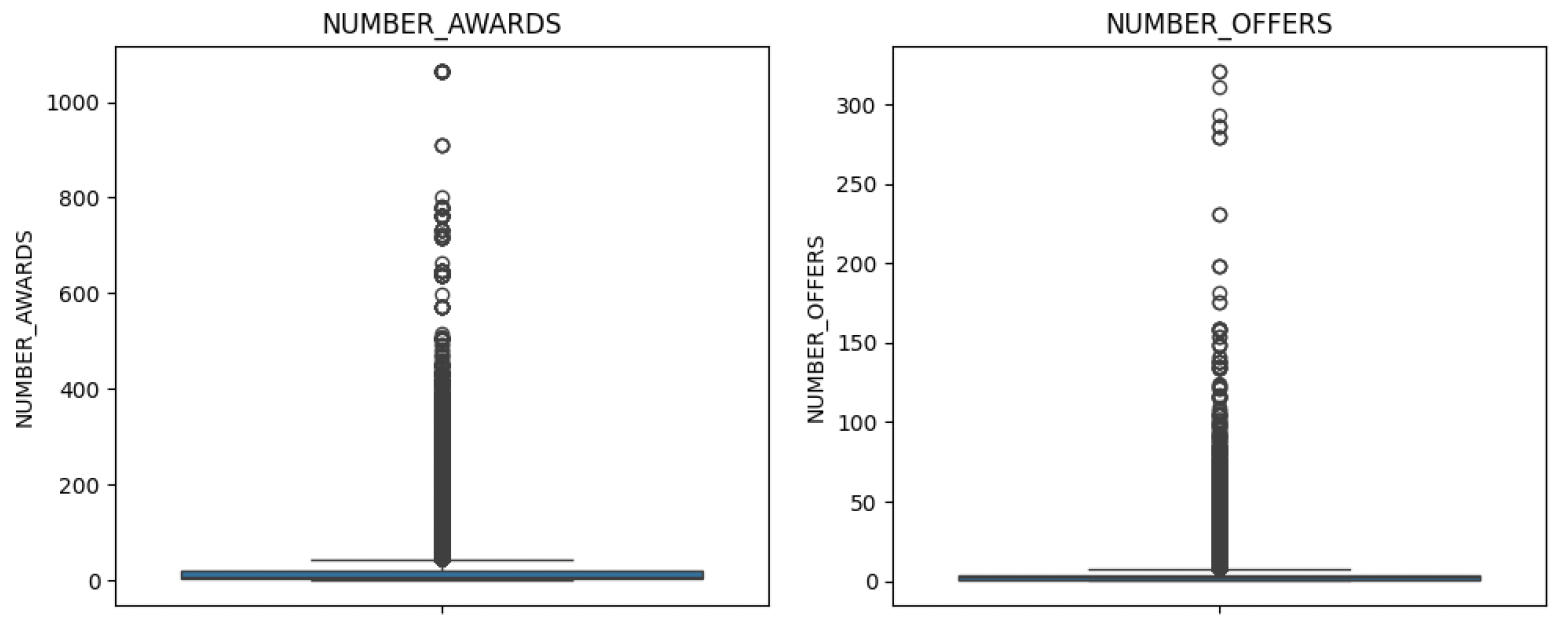
\includegraphics[width=.9\textwidth]{Imagenes/fig-015.png}	
\end{figure*} 

\paragraph{\textbf{Evaluación del balance de clases.}}

	La Figura \ref{fig:dispersion-variables-clasificacion} muestra el análisis univariable de las características categóricas, donde se evidenció un alto desbalance en la variable objetivo \texttt{CAE\_TYPE}, así como en otras como \texttt{ID\_TYPE},  \texttt{TYPE\_OF\_CONTRACT}, \texttt{TOP\_TYPE} y \texttt{B\_ON\_BEHALF}. 
%
	En particular, la característica \texttt{CAE\_TYPE}, utilizada como objetivo en la clasificación, muestra este patrón antes del balanceo, donde las clases 8 (54,860 registros) y 6 (46,841 registros) dominan el conjunto, mientras que categorías como 5 (508 registros) y 5a (12 registros) presentan escasa representación. 
Asimismo, las clases intermedias como la 3 (30,303 registros), la 1 (13,669 registros), la 4 (6,316 registros), así como las etiquetas ``n'' (2,944 registros)  y ``r'' (4,299 registros) también muestran una participación desigual.
%}

	Este patrón de desbalance se repite en otras variables. Por ejemplo, en \texttt{ID\_TYPE}, \linebreak \texttt{TYPE\_OF\_CONTRACT}, \texttt{TOP\_TYPE} y \texttt{B\_ON\_BEHALF}, entre otras. Por ejemplo, la mayoría de registros en \texttt{ID\_TYPE} pertenecen a la categoría 3, con más de 155,000 observaciones, frente a tan sólo 6,316 de la categoría 6. De manera similar, en \texttt{TOP\_TYPE}, la categoría ``ope'' domina el conjunto de datos con más de 159,000 casos, mientras que las demás categorías no superan los 2,500 registros.


	Dada esta distribución desigual, resulta esencial aplicar técnicas de balanceo antes del entrenamiento del modelo, con el fin de evitar que el algoritmo aprenda sesgos hacia las clases mayoritarias y de asegurar una representación adecuada de las clases minoritarias en la toma de decisiones.





\begin{figure*}[t]	
%	\begin{figure}[ht]
		\caption{Distribución univariables de las características seleccionadas para la clasificación.}	
	\label{fig:dispersion-variables-clasificacion}		
		\centering
		\begin{minipage}{.24\linewidth}
			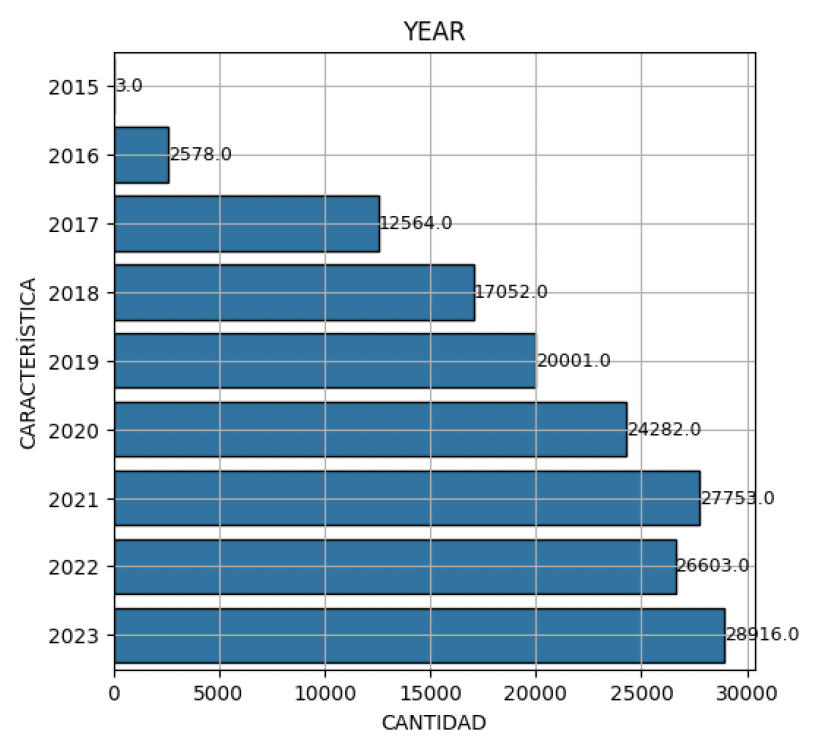
\includegraphics[width=1\linewidth]{Imagenes/univariable/fig-uni-0001}
		\end{minipage}%
		%	\hfill
		\begin{minipage}{.24\linewidth} 
			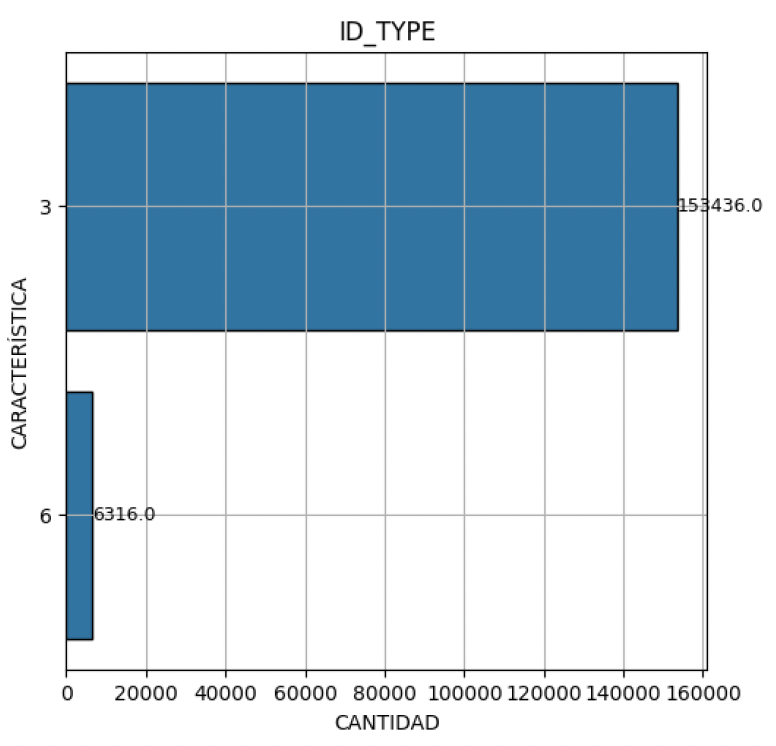
\includegraphics[width=1\linewidth]{Imagenes/univariable/fig-uni-0002}
		\end{minipage}
		%	\hfill
		\begin{minipage}{.24\linewidth} 
			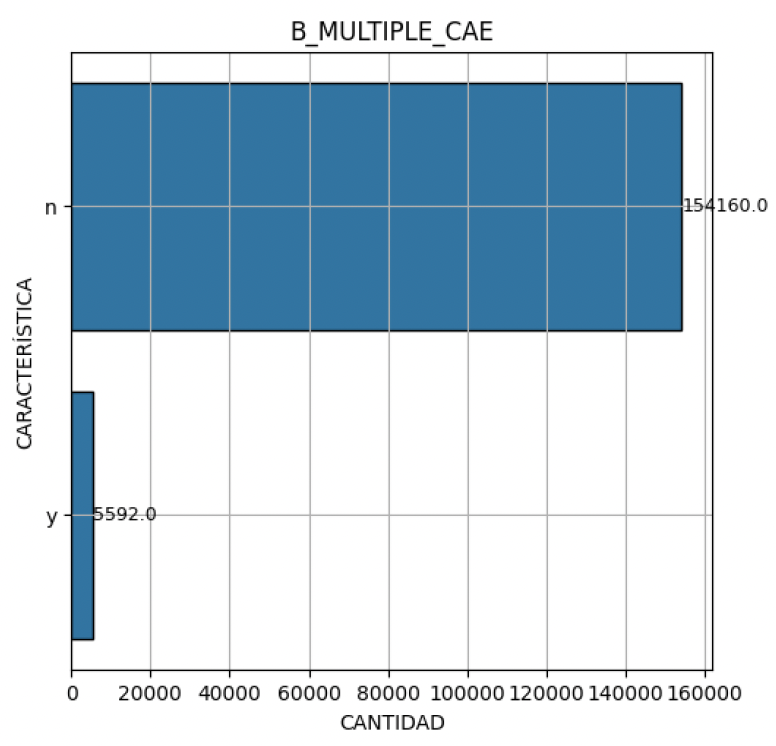
\includegraphics[width=1\linewidth]{Imagenes/univariable/fig-uni-0003}
		\end{minipage}	
		%	\hfill
		\begin{minipage}{.24\linewidth} 
			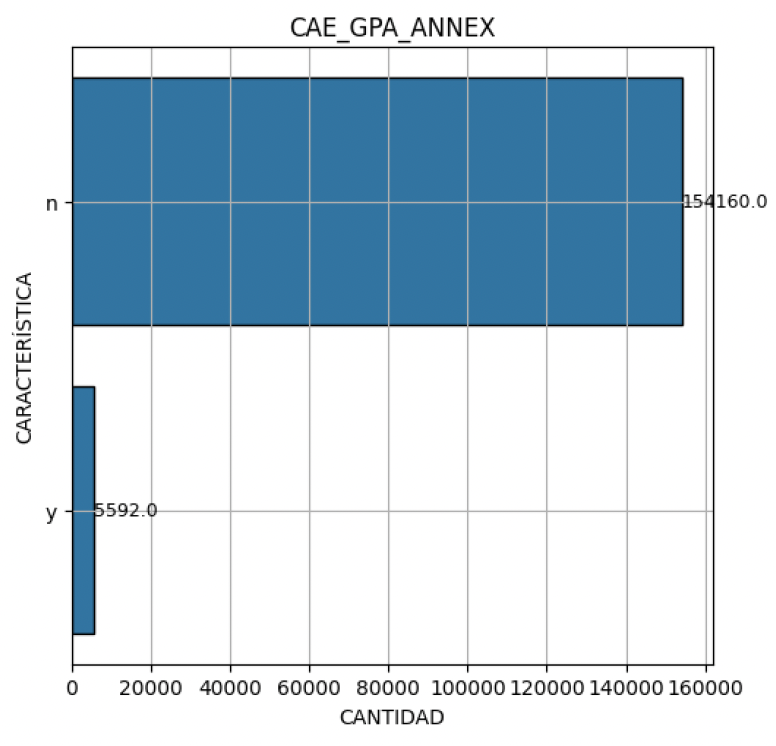
\includegraphics[width=1\linewidth]{Imagenes/univariable/fig-uni-0004}
		\end{minipage}
		\hfill
		\begin{minipage}{.24\linewidth} 
			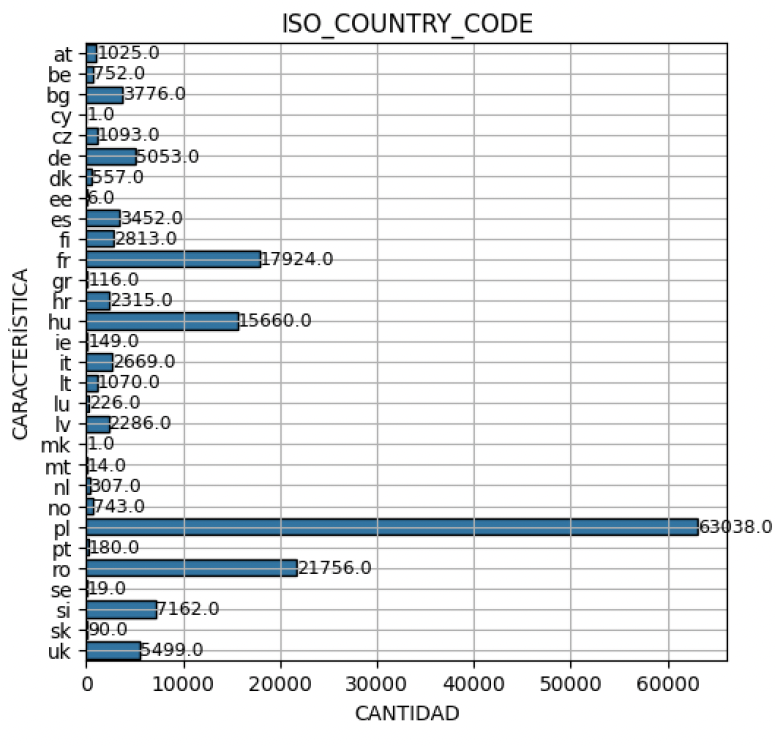
\includegraphics[width=1\linewidth]{Imagenes/univariable/fig-uni-0005}
		\end{minipage}
		%
		\begin{minipage}{.24\linewidth} 
			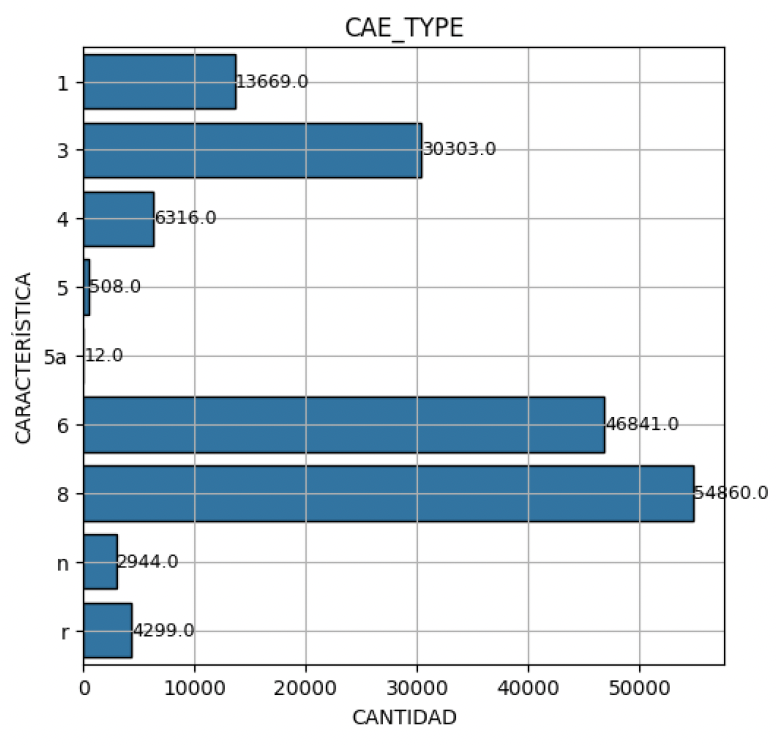
\includegraphics[width=1\linewidth]{Imagenes/univariable/fig-uni-0006}
		\end{minipage}
		%
		\begin{minipage}{.24\linewidth} 
			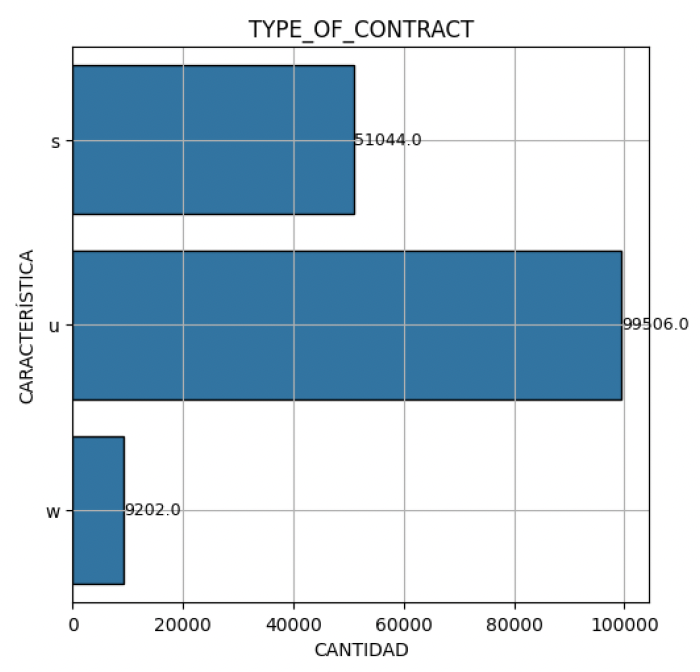
\includegraphics[width=1\linewidth]{Imagenes/univariable/fig-uni-0009}
		\end{minipage}
		%
		\begin{minipage}{.24\linewidth} 
			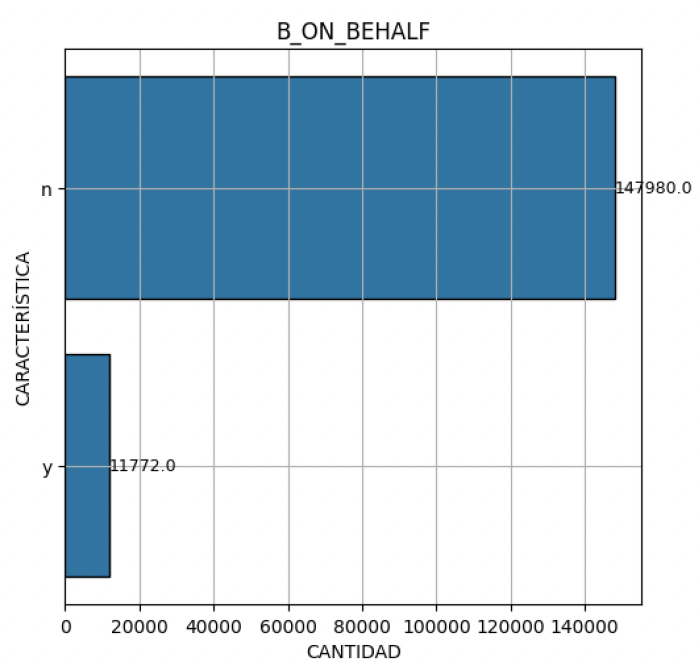
\includegraphics[width=1\linewidth]{Imagenes/univariable/fig-uni-0008}
		\end{minipage}
		\hfill
		%
		\begin{minipage}{.24\linewidth} 
			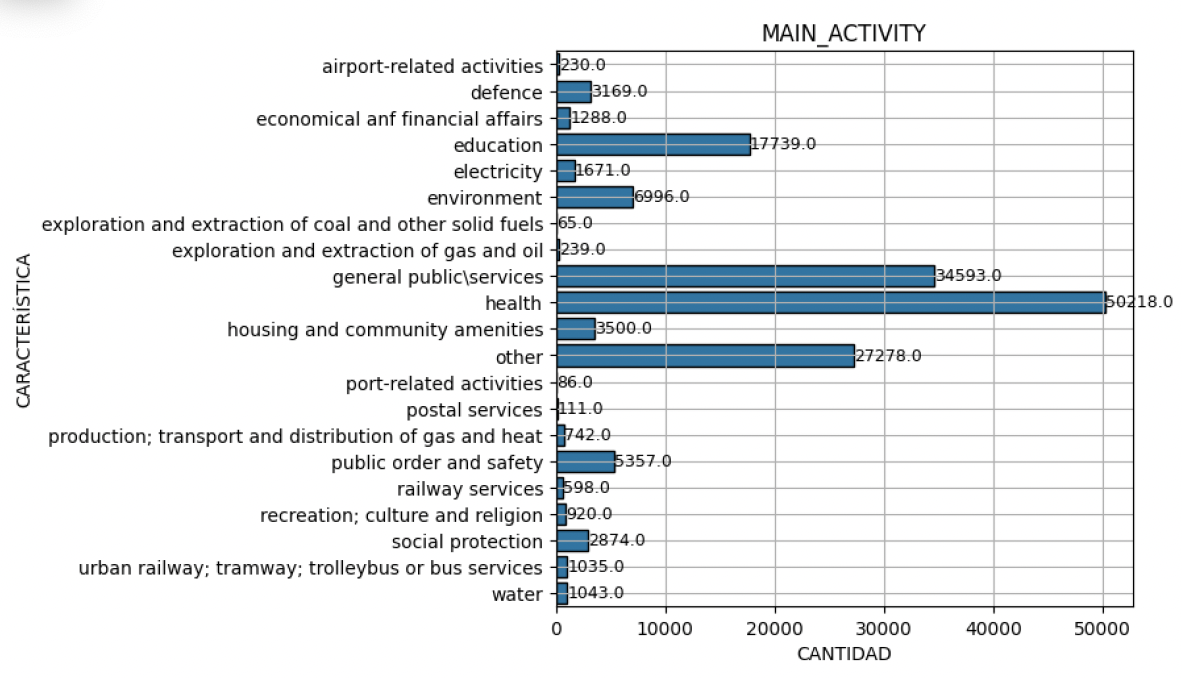
\includegraphics[width=1.3\linewidth]{Imagenes/univariable/fig-uni-0007}
		\end{minipage}
		%
		\begin{minipage}{.24\linewidth} 
			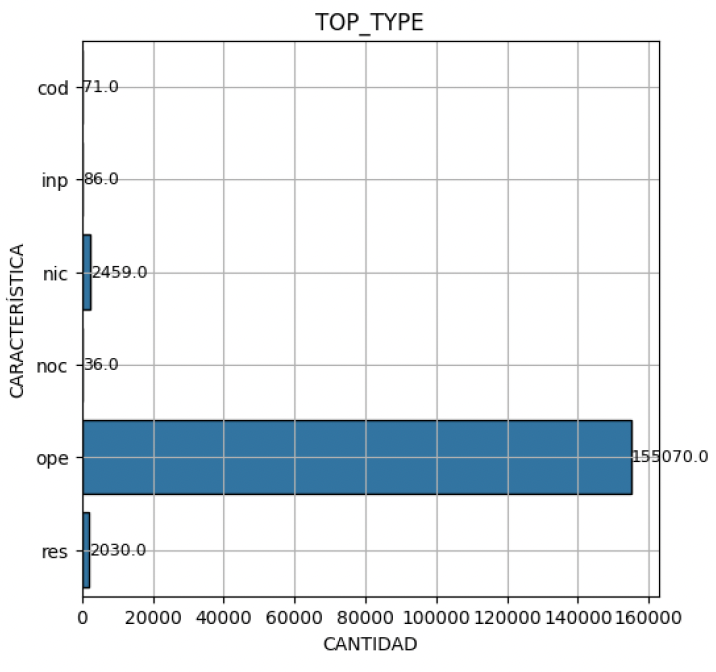
\includegraphics[width=1\linewidth]{Imagenes/univariable/fig-uni-0010}
		\end{minipage}
		%
		\begin{minipage}{.24\linewidth} 
			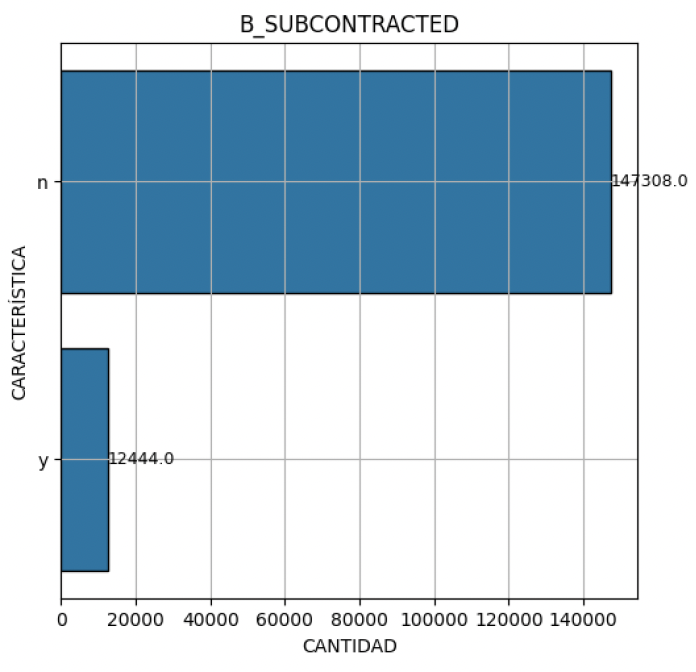
\includegraphics[width=1\linewidth]{Imagenes/univariable/fig-uni-0011}
		\end{minipage}
		%
		\begin{minipage}{.24\linewidth} 
			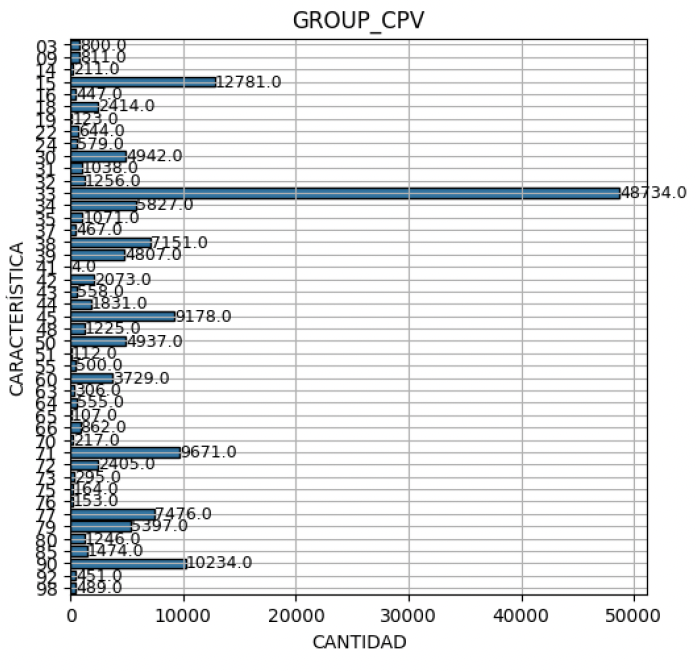
\includegraphics[width=1\linewidth]{Imagenes/univariable/fig-uni-0012}
		\end{minipage}
	\end{figure*}	

\subsection*{Data preparation}

\paragraph{\textbf{Balanceo de datos.}}
%
	Para mitigar el desbalance observado en la variable \texttt{CAE\_TYPE}, se aplicó \texttt{RandomOverSampler} de la biblioteca \textit{imbalanced-learn} en Python (\texttt{random\_state=42}), que duplica aleatoriamente instancias de las clases minoritarias hasta equiparar la distribución. Esta técnica fue preferida sobre SMOTE~\cite{chawla2002smote} porque el conjunto de datos contiene variables codificadas mediante \textit{OneHotEncoder} cuyos valores son estrictamente binarios; SMOTE generaría valores intermedios incompatibles con su naturaleza discreta \cite{geron2019hands,raschka2020python}.

\textbf{Nota metodológica.} El balanceo se aplicó sobre el conjunto completo, previo a la partición entrenamiento/prueba, lo que infla moderadamente las métricas. El balanceo se realizó sobre \texttt{CAE\_TYPE}; \texttt{SME\_WIN} presenta distribución 81.8\,\% positivos / 18.2\,\% negativos.

	Tras el balanceo, cada categoría de \texttt{CAE\_TYPE} contó con 54,860 registros, logrando una distribución uniforme. 
Debido a la correlación entre \texttt{CAE\_TYPE} y otras variables, 13 de las 16 características de clasificación se vieron afectadas por el re-muestreo, mientras que \linebreak \texttt{B\_CONTRACTOR\_SME},  \texttt{GROUP\_DURATION} y \texttt{GROUP\_VALUE\_EURO} permanecieron sin cambios.

\paragraph{\textbf{Decodificación para el sistema de reglas.}}

	Para el sistema de sugerencias basado en reglas, se generó una vista \emph{decodificada} de las variables categóricas previamente transformadas mediante \textit{OneHotEncoder}. 
Mientras el modelo de aprendizaje automático mantiene la versión numérica codificada, el sistema de reglas utiliza la representación categórica original, lo que facilita la interpretación de los resultados. 
La Figura \ref{fig:onehotencoder-inverso} muestra las instrucciones ejecutadas para la decodificación
 \texttt{OneHotEncoder}, preservando el tipo original de cada variable (\texttt{YEAR}, \texttt{CAE\_TYPE}, \texttt{ISO\_COUNTRY\_CODE}, \texttt{TYPE\_OF\_CONTRACT}, entre otras). 
Este proceso permite que las recomendaciones se expresen en términos comprensibles para los usuarios del sistema, manteniendo coherencia entre ambas vistas del conjunto de datos.

%\begin{figure}[H]
\begin{figure}[htb]	
	\caption{Instrucciones para la reversión de OneHotEncoding}	
	\label{fig:onehotencoder-inverso}	
	%	\centering
	\begin{verbatim}
		def decode_one_hot(df: pd.DataFrame, prefix: str) -> pd.DataFrame:
		decoded = df[df.columns[df.columns.str.startswith(prefix)]].idxmax(axis=1)
		decoded_column = decoded.str.split('_').str[-1]
		return pd.DataFrame({prefix: decoded_column})
		
		decoded_year = decode_one_hot(df_final_details, 'YEAR')
		decoded_cae_type = decode_one_hot(df_final_details, 'CAE_TYPE')
		decoded_b_multiple_cae = decode_one_hot(df_final_details, 'B_MULTIPLE_CAE')
		decoded_cae_gpa_annex = decode_one_hot(df_final_details, 'CAE_GPA_ANNEX')
		decoded_b_on_behalf = decode_one_hot(df_final_details, 'B_ON_BEHALF')
		decoded_id_type = decode_one_hot(df_final_details, 'ID_TYPE')
		decoded_iso_country_code = decode_one_hot(df_final_details, 'ISO_COUNTRY_CODE')
		decoded_top_type = decode_one_hot(df_final_details, 'TOP_TYPE')
		decode_type_of_contract = decode_one_hot(df_final_details, "TYPE_OF_CONTRACT")
		decode_b_subcontracted = decode_one_hot(df_final_details, "B_SUBCONTRACTED")
		decode_main_activity = decode_one_hot(df_final_details, "MAIN_ACTIVITY")
		decode_group_cpv= decode_one_hot(df_final_details, "GROUP_CPV")	
	\end{verbatim}
	
\end{figure}


\paragraph{\textbf{Generación de conjunto de datos normalizado.}}

	Finalizadas las tres iteraciones, se genera un conjunto de datos normalizado en formato \texttt{.parquet}. Este archivo consolidado es el resultado de todo el procesamiento previo y garantiza que los datos sean consistentes, estructurados y libres de ruido, optimizando así su uso en el entrenamiento del modelo de aprendizaje automático.

\subsection{Modeling}\label{sec:fase7}

Tras la preparación y depuración de los datos, el siguiente paso es la construcción del modelo de aprendizaje automático. En el contexto de licitaciones públicas, este modelo busca identificar patrones en la adjudicación de contratos, permitiendo generar sugerencias basadas en características relevantes de cada proceso de contratación.

Del conjunto de datos total, el 100~\% de ellos serán considerados para el modelado; es decir, un total de  159,752 registros, los cuales son necesarios dividirlos  de la siguiente manera. 

\begin{itemize}
	\item 70~\% = En datos de entrenamiento
	\item 15~\% = En datos de evaluación
	\item 15~\% = En datos de prueba
\end{itemize}

Los datos de entrenamiento se emplean para construir el modelo, mientras que los datos de evaluación permiten ajustar los hiperparámetros y controlar el sobreentrenamiento durante el proceso. Finalmente, los datos de prueba se utilizan para evaluar el rendimiento final del modelo, mediante métricas de clasificación que reflejen su capacidad predictiva.

En este estudio, se han aplicado los algoritmos \textit{Random Forest} y \textit{Gradient Boosting Classifier}, que se ajustan adecuadamente en el contexto de licitación \cite{FigueroaGomez2024}.


	Los modelos fueron evaluados mediante validación cruzada estratificada ($k=10$ folds) con \texttt{RandomOverSampler} aplicado exclusivamente sobre el conjunto de entrenamiento de cada fold. Se reportan media $\pm$ desviación estándar de accuracy, precision, recall, F1-macro y AUC-ROC (Exp.~B2).

	Con los modelos entrenados y validados mediante este proceso, se procedió a la fase de evaluación para analizar cuantitativamente el rendimiento de cada clasificador.

\paragraph{\textbf{Diseño experimental.}}


Se definieron dos experimentos que comparten el mismo conjunto de entrada, pero difieren en la variable objetivo: (A) \texttt{MAIN\_ACTIVITY} y (B) \texttt{SME\_WIN}, variable binaria que indica si al menos un lote fue adjudicado a una pyme. Se excluyó \texttt{NUMBER\_TENDERS\_SME} para evitar fuga conceptual.
%
Se empleó validación cruzada estratificada (k=10) para selección/comparación de modelos y se reservó un conjunto de prueba para evaluación final.
	
\subsection{Evaluation}\label{sec:fase8}

	En esta fase se evalúa la capacidad predictiva, la estabilidad y la eficiencia computacional de los modelos desarrollados. 
Para ello, se consideran matrices de confusión por clase, métricas globales de rendimiento 
(\textit{accuracy}, \textit{precision}, \textit{recall} y \textit{F1-score}) y los tiempos de entrenamiento como indicadores del coste computacional asociado a cada algoritmo.

Las ejecuciones experimentales se realizaron en un equipo de uso personal, cuyas especificaciones se presentan en la Tabla~\ref{tab:caracteristicas_entorno}.
Estas características permiten contextualizar el desempeño computacional reportado y facilitan la reproducibilidad de los resultados.

\begin{table}[H]
	\small
	\setlength{\tabcolsep}{7pt}
	\renewcommand{\arraystretch}{1.3} % Aumenta el espacio entre filas	
	\centering
	\caption[Características del entorno de prueba]{Características del entorno de prueba}
	\label{tab:caracteristicas_entorno}
	\begin{tabular}{cp{5.5cm}cc}
		\hline
		\textbf{Sistema Operativo} & \textbf{Procesador} & \textbf{RAM} & \textbf{Almacenamiento} \\
		\hline
		Windows 11 & AMD Ryzen 7 5700G with Radeon Graphics @ 3.80\,GHz (8 núcleos, 16 hilos) & 16\,GB & 1\,TB \\
		\hline
	\end{tabular}
\end{table}
	

\paragraph{\textbf{Evaluación del modelo.}}

%
Para la validación de los modelos de clasificación multiclase utilizados en este estudio, se emplea la técnica de matriz de confusión. Esta herramienta permite analizar detalladamente el desempeño del modelo, comparando las predicciones realizadas con los valores reales del conjunto de prueba. En este contexto, se utilizarán matrices de confusión {desfragmentadas}; es decir, representadas de forma completa para cada clase, permitiendo un análisis interno exhaustivo.

La matriz de confusión no solo proporciona una visión global del comportamiento del modelo, sino que también permite calcular métricas fundamentales como la \textit{precisión}, el \textit{recall} (sensibilidad), la \textit{exactitud} y la \textit{F1-score}. Estas métricas se derivan de los siguientes componentes, que en el caso multiclase se calculan por cada clase (\textit{one-vs-all}):

\begin{itemize}
	\item \textbf{TP} (\textit{True Positive}): Casos correctamente clasificados como positivos (pertenecen a la clase y fueron predichos como tal).
	\item \textbf{TN} (\textit{True Negative}): Casos correctamente clasificados como negativos (no pertenecen a la clase y fueron correctamente excluidos).
	\item \textbf{FP} (\textit{False Positive}): Casos que no pertenecen a la clase, pero fueron clasificados incorrectamente como positivos.
	\item \textbf{FN} (\textit{False Negative}): Casos que pertenecen a la clase, pero fueron clasificados incorrectamente como negativos.
\end{itemize}

En el caso multiclase, estos valores se computan por cada clase, considerando a cada una como clase positiva mientras el resto actúan como negativas. Esto permite evaluar de forma más precisa el rendimiento global y por clase del modelo.


\paragraph{\textbf{Experimento A.}}

	Este experimento busca sugerir la actividad principal de la entidad contratante (\texttt{MAIN\_ACTIVITY}). Las métricas por clase obtenidas a partir de las matrices de confusión se muestran en la Tabla~\ref{tab:experimento-a-matriz-confusion}, los cuales se derivan directamente de las predicciones del modelo.  En términos generales, ambos modelos presentan altos valores de \textit{TP} en las clases mayoritarias,  como \texttt{general public services} (20,010 TP) y \texttt{health} (11,493 TP), lo que se refleja en las diagonales predominantes de
	las matrices de confusión mostradas en la Figura \ref{fig:experimento-a-matrices-rf-gb}: en (a), el modelo \textit{Random Forest}, mientras que en (b), el modelo \textit{Gradient Boosting}.
	 Sin embargo, se observan dificultades en clases minoritarias como \textit{port-related activities} y \textit{postal services}, donde se reportan mayores valores de \textit{FP} y \textit{FN}, 
%	  
	 	lo que implica que los modelos tienen dificultades para distinguir correctamente entre estas categorías menos frecuentes.



\begin{figure*}[t]
	\caption{Matrices de confusión de los modelos \textit{Random Forest} y \textit{Gradient Boosting} para el experimento A.}
	\label{fig:experimento-a-matrices-rf-gb}	
	\centering	
	\begin{minipage}{0.48\textwidth} % 48% del ancho de la página
	
\includegraphics[width=\textwidth]{Imagenes/capitulo_tres/GA/RandomForest}		
	\\
		\centering\textit{(a)}
	\end{minipage}%
		\hfill
	\begin{minipage}{0.48\textwidth} % 48% del ancho de la página
	
\includegraphics[width=\textwidth]{Imagenes/capitulo_tres/GA/GradientBoosting}		
	\\
		\centering\textit{(b)}		
	\end{minipage}	
\end{figure*}



Algunas diferencias sutiles encontradas en los algoritmos se presenta a continuación:

\begin{itemize}
	\item En la clase \textit{education}, Random Forest presenta 3,960 verdaderos positivos y Gradient Boosting 3,956, con ligeras diferencias en los valores de FN y FP, lo que significa que existe un rendimiento comparable entre ambos modelos.
	
	\item En la clase \textit{electricity}, Gradient Boosting obtiene una ligera ventaja , con 1,591 TP frente a 1,586 de Random Forest. Además, reduce ligeramente el número de falsos negativos (606 frente a 611), lo que sugiere una leve mejora en la capacidad de detección.
	
	\item En clases más complejas como \textit{other}, {Gradient Boosting} mejora la clasificación, tanto en la clasificación de instancias positivas como negativas, con 16,330 verdaderos positivos frente a 16,319 en {Random Forest} y una reducción de 11 unidades en los falsos negativos, lo que refuerza su capacidad para manejar clases con mayor variabilidad interna.	
	
\end{itemize}


Sin embargo, las diferencias globales entre ambos modelos no son sustanciales en términos de precisión por clase. 
%
%
	Ambos modelos muestran signos de desbalance de clases en sus predicciones, fenómeno que se refleja en la concentración de errores en clases poco representadas.
%	


\begin{table*}[t]
	\centering
%	\small
	\scriptsize
	\renewcommand{\arraystretch}{1.3} % Aumenta el espacio entre filas
	\setlength{\tabcolsep}{7pt}
\caption{Experimento A: Métricas TP, TN, FP y FN por clase con \textit{Random Forest} y \textit{Gradient Boosting}.}	
	\label{tab:experimento-a-matriz-confusion}	
	\begin{adjustbox}{max width=\textwidth}	
		\begin{tabular}{p{4cm}rrrrcrrrr} 			
			\hline
			\multicolumn{1}{c}{\multirow{2}{*}{\textbf{\textsc{CLASES}}}} & \multicolumn{4}{c}{\textbf{\textsc{Random Forest}}} & \multirow{2}{*}{} & \multicolumn{4}{c}{\textbf{\textsc{Gradient Boosting}}} \\ \cline{2-5} \cline{7-10}
			{} & \textbf{\textsc{TP}} & \textbf{\textsc{TN}} & \textbf{\textsc{FP}} & \textbf{\textsc{FN}} & & \textbf{\textsc{TP}} & \textbf{\textsc{TN}} & \textbf{\textsc{FP}} & \textbf{\textsc{FN}} \\ \cline{1-10} %\cline{7-10}
			airport-related activities & 126 & 73,628 & 124 & 183 & & 126 & 73,628 & 124 & 183 \\ 
			defense & 789 & 72,261 & 178 & 833 & & 787 & 72,262 & 177 & 835 \\ 
			economic and financial affairs & 985 & 72,383 & 120 & 573 & & 985 & 72,384 & 119 & 573 \\ 
			education & 3,960 & 67,350 & 722 & 2,029 & & 3,956 & 67,353 & 719 & 2,033 \\ 
			electricity & 1,586 & 71,398 & 466 & 611 & & 1,591 & 71,385 & 479 & 606 \\ 
			environment & 715 & 71,410 & 451 & 1,485 & & 713 & 71,413 & 448 & 1,487 \\ 
			exploration and extraction of coal and other solid fuels & 27 & 73,941 & 25 & 68 & & 24 & 73,956 & 10 & 71 \\ 
			exploration and extraction of gas and oil & 164 & 73,702 & 79 & 116 & & 164 & 73,702 & 79 & 116 \\ 
			general public services & 20,010 & 54,051 & 0 & 0 & & 20,010 & 54,051 & 0 & 0 \\ 
			health & 11,493 & 62,568 & 0 & 0 & & 11,493 & 62,568 & 0 & 0 \\ 
			housing and community amenities & 522 & 72,778 & 183 & 578 & & 526 & 72,774 & 187 & 574 \\ 
			other & 16,319 & 49,551 & 6,732 & 1,459 & & 16,330 & 49,544 & 6,739 & 1,448 \\ 
			port-related activities & 28 & 73,942 & 17 & 74 & & 28 & 73,942 & 17 & 74 \\ 
			postal services & 49 & 73,913 & 8 & 91 & & 49 & 73,913 & 8 & 91 \\ 
			production; transport and distribution of gas and heat & 449 & 72,957 & 134 & 521 & & 453 & 72,948 & 143 & 517 \\ 
			public order and safety & 1,496 & 70,888 & 330 & 1,347 & & 1,496 & 70,892 & 326 & 1,347 \\ 
			railway services & 310 & 73,035 & 258 & 458 & & 303 & 73,041 & 252 & 465 \\ 
			recreation; culture and religion & 61 & 73,632 & 9 & 359 & & 61 & 73,632 & 9 & 359 \\ 
			social protection & 951 & 72,352 & 217 & 541 & & 949 & 72,356 & 213 & 543 \\ 
			urban railway; tramway; trolleybus or bus services & 895 & 71,140 & 1,585 & 441 & & 895 & 71,140 & 1,585 & 441 \\ 
			water & 747 & 71,961 & 741 & 612 & & 747 & 71,961 & 741 & 612 \\ 
			\hline
		\end{tabular}
	\end{adjustbox}		
\end{table*}




\paragraph{\textbf{Experimento B.}}


	En este caso, el modelo predice si una licitación será adjudicada a una pyme (\texttt{SME\_WIN}\,=\,1) o no (\texttt{SME\_WIN}\,=\,0). Los resultados se resumen en la Tabla~\ref{tab:experimento-b-matriz-confusion}. Ambos modelos presentan un desempeño sobresaliente en la clase predominante \texttt{(-0.2, 67.611]}, mientras que las clases de menor frecuencia muestran mayores errores de clasificación. Gradient Boosting evidencia ligeras mejoras respecto a Random Forest en clases intermedias, aunque estas diferencias no resultan sustanciales.



Este experimento se diseñó para predecir la adjudicación de licitaciones a pymes (\texttt{SME\_WIN}), como clasificación binaria. La variable se derivó de \texttt{B\_CONTRACTOR\_SME}: \texttt{SME\_WIN\,=\,1} si al menos un lote fue adjudicado a una pyme. Distribución: 81.8\,\% positivos, gestionada con \texttt{RandomOverSampler} inside-fold. Se comparó los rendimientos en la predicción multiclase de los dos modelos Random Forest y Gradient Boosting. Las métricas TP, TN, FP, FN se presentan en la Tabla~\ref{tab:experimento-b-matriz-confusion}, mientras que las respectivas matrices de confusión se ilustran en la Figura \ref{fig:experimento-b-matrices-rf-gb}:
en (a), el modelo \textit{Random Forest}, mientras que en (b), el modelo \textit{Gradient Boosting}.

Los resultados del Experimento~B2 (\texttt{SME\_WIN}) muestran un rendimiento sólido: Precision\,=\,$0.8877 \pm 0.0022$, Recall\,=\,$0.6808 \pm 0.0040$, F1\,=\,$0.7706 \pm 0.0025$ y AUC\,=\,$0.7096 \pm 0.0050$. La alta precisión (88.8\,\%) implica que el modelo acierta en casi 9 de cada 10 predicciones favorables a pyme. La estabilidad es notable: std(F1)\,=\,0.0025 sobre 10 folds.

Las clases con menos instancias (\texttt{(134.222, 200.833]}, \texttt{(600.5, 667.111]} y \texttt{(933.556, 1000.167]}) presentan mayor dificultad de clasificación para ambos modelos, con varios valores FN altos en relación al número total de casos.

En el intervalo \texttt{(67.611, 134.222]}, el modelo Gradient Boosting presenta una leve mejora en el rendimiento, alcanzando 368 verdaderos positivos frente a los 365 obtenidos por Random Forest, reduciendo en tres la cantidad de falsos negativos, lo cual se refleja en una mayor concentración en la diagonal de la matriz de confusión.


A continuación, se presenta la comparación de los resultados de los modelos:

\begin{itemize}
	\item Random Forest y Gradient Boosting muestran resultados casi idénticos en la mayoría de clases. No obstante, GB muestra una ligera mejora de precisión en clases como \texttt{(67.611, 134.222]} y \texttt{(933.556, 1000.167]} al reducir levemente los falsos negativos.
	
	\item Las matrices de confusión muestran una diagonal dominante en ambas figuras, lo que indica que los modelos están prediciendo correctamente en la mayoría de los casos. Sin embargo, también se observan leves dispersiones fuera de la diagonal en clases minoritarias, indicando posibles errores de clasificación (confusiones entre clases contiguas).
\end{itemize}

%\begin{table}[htb]
\begin{table*}[t]	
	\centering
	\scriptsize
%	\small
	\setlength{\tabcolsep}{7pt}
	\renewcommand{\arraystretch}{1.3} % Aumenta el espacio entre filas
	\caption{Experimento B: Métricas TP, TN, FP y FN por clase con \textit{Random Forest} y \textit{Gradient Boosting}.}	
	\label{tab:experimento-b-matriz-confusion}
	\begin{adjustbox}{max width=\textwidth}
		\begin{tabular}{p{4cm}rrrrcrrrr}			
			\hline
			\multicolumn{1}{c}{\multirow{2}{*}{\textbf{\textsc{CLASES}}}} &
			 \multicolumn{4}{c}{\textbf{\textsc{Random Forest}}} & \multirow{2}{*}{} & \multicolumn{4}{c}{\textbf{\textsc{Gradient Boosting}}} \\ \cline{2-5} \cline{7-10}			
			 
			{} & \textbf{TP} & \textbf{TN} & \textbf{FP} & \textbf{FN} & & \textbf{TP} & \textbf{TN} & \textbf{FP} & \textbf{FN} \\ \cline{1-10} %\cline{7-10}
			(-0.2, 67.611] & 72,937 & 403 & 669 & 52 & & 72,937 & 406 & 666 & 52 \\ 
			(1133.389, 1200.0] & 7 & 74,034 & 5 & 15 & & 7 & 74,034 & 5 & 15 \\ 
			(134.222, 200.833] & 6 & 74,019 & 0 & 36 & & 6 & 74,019 & 0 & 36 \\ 
			(200.833, 267.444] & 0 & 74,059 & 0 & 2 & & 0 & 74,059 & 0 & 2 \\ 
			(334.056, 400.667] & 0 & 74,054 & 0 & 7 & & 0 & 74,054 & 0 & 7 \\ 
			(467.278, 533.889] & 17 & 74,016 & 7 & 21 & & 17 & 74,016 & 7 & 21 \\ 
			(600.5, 667.111] & 0 & 74,060 & 0 & 1 & & 0 & 74,060 & 0 & 1 \\ 
			(67.611, 134.222] & 365 & 73,073 & 40 & 583 & & 368 & 73,073 & 40 & 580 \\ 
			(933.556, 1000.167] & 8 & 74,049 & 0 & 4 & & 8 & 74,049 & 0 & 4 \\ \hline
		\end{tabular}
	\end{adjustbox}

\end{table*}


\begin{figure*}[t]	
	\caption{Matrices de confusión de los modelos \textit{Random Forest} y \textit{Gradient Boosting} para el experimento B.}
	\label{fig:experimento-b-matrices-rf-gb}	
	\centering	
	\begin{minipage}{0.48\textwidth} % 48% del ancho de la página
	
\includegraphics[width=\textwidth]{Imagenes/capitulo_tres/GB/RandomForest}		
		\\
		\centering\textit{(a)}
	\end{minipage}%
	\hfill
	\begin{minipage}{0.48\textwidth} % 48% del ancho de la página
	
\includegraphics[width=\textwidth]{Imagenes/capitulo_tres/GB/GradientBoosting}		
		\\
		\centering\textit{(b)}		
	\end{minipage}	
\end{figure*}




	Los datos presentados en las Tablas \ref{tab:experimento-a-matriz-confusion}	y \ref{tab:experimento-b-matriz-confusion}  servirán para calcular los porcentajes decumplimiento de las métricas \textit{accuracy, precision, recall} y  \textit{f1--score}.



\paragraph{\textbf{Importancia de los predictores en los modelos de clasificación.}}
	Es importante analizar el impacto de las caracter\'isticas de entrada en los modelos de clasificaci\'on desarrollados mediante \textit{Random Forest} y {Gradient Boosting}, en el contexto de los Experimentos A y B. La Tabla~\ref{tab:importancia_predictores} presenta los valores de importancia asignados a cada predictor en ambos experimentos, permitiendo identificar las variables que mayor influencia tienen en el proceso de predicci\'on.

\begin{table*}[t]		
	
	\small
	\setlength{\tabcolsep}{7pt}
		\renewcommand{\arraystretch}{1.3} % Aumenta el espacio entre filas
		\caption{Importancia de los  predictores en los modelos}	
			\label{tab:importancia_predictores}
\centering		
	\begin{adjustbox}{max width=\textwidth}		
		\begin{tabular}{p{3.5cm}rrcrr}			
		\hline
		\multicolumn{1}{c}{\multirow{2}{*}{\textbf{\textsc{Clasificador}}}} & \multicolumn{2}{c}{\textbf{\textsc{Experimento A}}}          &         & \multicolumn{2}{c}{\textbf{Experimento B}} \\ \cline{2-3} \cline{5-6} 
		\multicolumn{1}{c}{} &
		\multicolumn{1}{p{1.5cm}}{\textbf{\textsc{Random Forest}}} &
		\multicolumn{1}{p{2cm}}{\textbf{\textsc{Gradient Boosting}}} & &
		\multicolumn{1}{p{1.5cm}}{\textbf{\textsc{Random Forest}}} &
		\multicolumn{1}{p{2cm}}{\textbf{\textsc{Grandient Boosting}}} \\ \hline
		\texttt{MAIN\_ACTIVITY\_general public\_services} & \textbf{0.321547}      & 0.018176                   & & 0.043592               & 0.008024                   \\ %\hline
		\texttt{MAIN\_ACTIVITY\_health}                   & 0.163550               & 0.005850        &           & 0.024853               & 0.020555                   \\ %\hline
		\texttt{NUMBER\_AWARDS}                           & 0.096012               & 0.215469              &     & \textbf{0.223706}      & 0.196990                   \\ %\hline
		\texttt{LOTS\_NUMBER}                             & 0.086634               & \textbf{0.245214}     &     & 0.197382               & 0.143185                   \\ %\hline
		\texttt{NUMBER\_OFFERS}                           & 0.058054               & 0.137373            &       & 0.134636               & \textbf{0.273736}          \\ %\hline
		\texttt{GROUP\_CPV\_33}                           & 0.070151               & 0.010685           &        & 0.023014               & 0.010808                   \\ %\hline
		\texttt{NUMBER\_TENDERS\_SME}                     & 0.048584               & 0.152201     &              & 0.113017               & 0.244014                   \\ %\hline
		\texttt{CAE\_TYPE\_4}                             & 0.052990               & 0.009884            &       & 0.042516               & 0.002140                   \\ %\hline
		\texttt{CAE\_TYPE\_3}                             & 0.033222               & 0.017911            &       & 0.021146               & 0.028675                   \\ %\hline
		\texttt{CAE\_TYPE\_5}                            & 0.014599               & 0.002020             &      & 0.045162               & 0.000817                   \\ %\hline
		\texttt{GROUP\_CPV\_15}                           & 0.014559               & 0.050781          &         & 0.010516               & 0.001811                   \\ %\hline
		\texttt{ISO\_COUNTRY\_CODE\_lu}                   & 0.007542               & 0.000282       &            & 0.012956               & 0.000623                   \\ %\hline
		\texttt{B\_ON\_BEHALF\_n}                        & 0.009952               & 0.040915               &    & 0.038911               & 0.016911                   \\ %\hline
		\texttt{ISO\_COUNTRY\_CODE\_si}                  & 0.009129               & 0.025078           &        & 0.003416               & 0.003774                   \\ %\hline
		\texttt{B\_MULTIPLE\_CAE\_n}                      & 0.005365               & 0.024908              &     & 0.015455               & 0.013862                   \\ %\hline
		\texttt{TYPE\_OF\_CONTRACT\_w}                    & 0.004135               & 0.026261            &       & 0.025973               & 0.028177                   \\ %\hline
		\texttt{GROUP\_CPV\_45}                          & 0.003975               & 0.016991               &    & 0.023748               & 0.005897                   \\ \hline
	\end{tabular}
	\end{adjustbox}	

\end{table*}


\paragraph{\textbf{Tiempo de respuesta.}}

	Además del rendimiento predictivo, se evaluó la eficiencia computacional de los modelos mediante la medición de sus tiempos de entrenamiento. 
La Tabla~\ref{tab:tiempo_respuesta_ml} muestra los resultados obtenidos para ambos experimentos, evidenciando las diferencias significativas en el tiempo requerido por cada algoritmo.

\begin{table}[tb]	
	\caption{Tiempos de entrenamiento =10 folds por experimento y modelo. Entorno de ejecución: Google Colaboratory (CPU Intel Xeon, RAM 12\,GB). Todos los experimentos ejecutados en el mismo entorno para garantizar comparabilidad.}
	\label{tab:tiempo_respuesta_ml}
	\centering
	\small
	\setlength{\tabcolsep}{7pt}
	\renewcommand{\arraystretch}{1.3} % Aumenta el espacio entre filas	
	\begin{tabular}{ccc}\hline
\textbf{Experimento} & \textbf{Modelo} & \textbf{Tiempo ($k=10$ folds)} \\ \hline
\multirow{2}{*}{A} & Random Forest & 16.2 min \\ \cline{2-3}
& Gradient Boosting & 219.4 min \\ \hline
\multirow{2}{*}{B2} & Random Forest & 3.5 min \\ \cline{2-3}
& Gradient Boosting & 1.9 min \\ \hline
\end{tabular}
\end{table}


\subsection*{Análisis de resultados.}

A continuación, se presentan los hallazgos derivados de la interpretación de la importancia de características en los modelos aplicados a los dos experimentos definidos.

\paragraph{\textbf{Análisis del Experimento A.}}

%
En el Experimento A, el modelo RF asign\'o una importancia significativa a la caracter\'istica \texttt{MAIN\_ACTIVITY\_general public\_services}, con un valor de 0.3215, lo que indica que esta variable tuvo un rol determinante en la clasificaci\'on. En contraste, {Gradient Boosting} dio mayor peso a variables num\'ericas como \texttt{LOTS\_NUMBER} (0.2452) y \texttt{NUMBER\_AWARDS} (0.2155), mostrando un enfoque diferente en la selecci\'on de patrones relevantes.
%
{En conclusi\'on}, los modelos responden de forma distinta al mismo conjunto de datos: Random Forest se inclina por variables categóricas estructurales, mientras que Gradient Boosting prioriza indicadores numéricos relacionados con volumen y participación, lo que refleja una diferencia en la estrategia de aprendizaje de cada algoritmo.

\paragraph{\textbf{Análisis del Experimento B.}}
%
En el Experimento B se evidencia un cambio en la jerarqu\'ia de importancia. Para RF, la variable \texttt{NUMBER\_AWARDS} se posicion\'o como la m\'as relevante (0.2237), seguida de \texttt{LOTS\_NUMBER} (0.1974). Por su parte, {Gradient Boosting} destac\'o \texttt{NUMBER\_OFFERS} (0.2737) y \texttt{NUMBER\_TENDERS\_SME} (0.2440) como los principales predictores. Estos resultados indican que el cambio en la variable objetivo del modelo afecta la importancia relativa de las caracter\'isticas.
%
{En conclusi\'on}, el cambio en la etiqueta a predecir influye notablemente en la estructura del conocimiento aprendido por los modelos, lo cual demuestra la necesidad de seleccionar cuidadosamente las variables de entrada en función del objetivo del análisis.

\subsection*{Conclusiones}

El an\'alisis comparativo muestra que los modelos identifican patrones distintos dependiendo del experimento. Mientras que en el Experimento A predominaron las variables categ\'oricas asociadas a la actividad principal de la entidad contratante, en el Experimento B destacaron las variables num\'ericas relacionadas con el comportamiento cuantitativo del proceso licitatorio. Adem\'as, se confirma que \textit{Gradient Boosting} tiende a identificar relaciones no lineales y complejas con mayor eficacia, redistribuyendo el peso de las variables de manera m\'as focalizada que \textit{Random Forest}.

Esto resalta la importancia de seleccionar adecuadamente las variables de entrada seg\'un el objetivo del modelo y de evaluar distintos algoritmos para identificar el que mejor se ajusta a la naturaleza del problema.

	En conjunto, ambos modelos muestran buen desempeño en clases mayoritarias y dificultades en minoritarias, con ventaja de RF en F1-macro y AUC, y coste 32$\times$ inferior en Exp.\,A. La baja fidelidad LIME en Exp.\,B2 (R\textsuperscript{2}\,=\,0.16) motiva el uso de SHAP como trabajo futuro.

	
	
	\subsection{Deployment}\label{sec:fase9}
	
	En esta fase se pone a prueba el modelo entrenado y el sistema de sugerencias asociado en un entorno de ejecución controlado y reproducible, permitiendo su utilización directa desde código \textit{Python}. 
	El despliegue se realizó mediante la serialización del modelo final y su posterior carga en un entorno de ejecución que replica las condiciones definidas durante el entrenamiento y la evaluación.
	
	El modelo de aprendizaje automático se almacenó en formato \texttt{.pkl}, lo que permite su reutilización y ejecución sin necesidad de reentrenamiento. 
	A partir de este archivo, el modelo es cargado dinámicamente dentro de un script en \textit{Python}, donde se suministran instancias de prueba que respetan la estructura final del conjunto de datos generado en la fase de preparación, incluyendo normalización, codificación categórica y selección de características.
	
	El flujo de despliegue contempla la recepción de los datos de entrada en su representación numérica final, la generación de la predicción multiclase y el cálculo de las probabilidades asociadas a cada clase. 
	Este enfoque permite validar el comportamiento del modelo en condiciones equivalentes a un escenario operativo, asegurando la coherencia entre los resultados obtenidos en las fases experimentales y su ejecución posterior.
	
	
	
Con el fin de mejorar la claridad del proceso de decisión, 
se integra el módulo \textit{LIME} (\textit{Local Interpretable Model-agnostic Explanations}), que produce una explicación local de las características que más influyeron en la predicción del modelo.	 	Estas explicaciones se producen directamente desde el entorno de ejecución en \textit{Python}, permitiendo analizar el razonamiento del modelo sin depender de una interfaz gráfica.
		
	De forma complementaria, el despliegue 
integra un motor de reglas que opera sobre las variables categóricas restauradas mediante el proceso inverso del \textit{OneHotEncoder}, permitiendo producir sugerencias basadas tanto en el modelo de aprendizaje automático como en criterios semiestructurados derivados de las características originales de las licitaciones.	
	
	En conjunto, esta fase demuestra la viabilidad del uso del modelo y del sistema de sugerencias en un entorno reproducible basado en código, sentando las bases para una futura integración en arquitecturas más complejas o entornos productivos sin modificar el núcleo analítico del sistema.
	
	
	
	\paragraph{\textbf{Caso de prueba.}}
	
	Como parte del despliegue, se realizó una verificación funcional del sistema empleando un conjunto de características representativas, con el fin de confirmar la consistencia entre el preprocesamiento aplicado en entrenamiento y el utilizado en producción. La Tabla~\ref{tab:datos_prediccion} presenta los valores de entrada utilizados en esta prueba, los cuales reflejan la estructura final del conjunto de datos procesado durante la fase de preparación.
	

\begin{table*}[t]
	\small
	\setlength{\tabcolsep}{7pt}
	\renewcommand{\arraystretch}{1.2} % Aumenta el espacio entre filas
	\caption{Datos a clasificar}
	\label{tab:datos_prediccion}
	\centering		
	\begin{adjustbox}{max width=\textwidth}		
		\begin{tabular}{lcc}
			\hline
			\multicolumn{1}{c}{\textbf{\textsc{Características}}} & \multicolumn{2}{c}{\textbf{\textsc{Valores de entrada}}} \\ \hline
			\texttt{B\_MULTIPLE\_CAE\_n} & 0 & 1 \\ 
			\texttt{B\_ON\_BEHALF\_n} & 0 & 1 \\ 
			\texttt{GROUP\_CPV\_45} & 0 & 0 \\ 
			\texttt{GROUP\_CPV\_15} & 0 & 1 \\ 
			\texttt{GROUP\_CPV\_33} & 1 & 0 \\ 
			\texttt{TYPE\_OF\_CONTRACT\_w} & 1 & 1 \\ 
			\texttt{MAIN\_ACTIVITY\_health} & 0 & 1 \\ 
			\texttt{ISO\_COUNTRY\_CODE\_si} & 0 & 0 \\ 
			\texttt{NUMBER\_AWARDS} & 3 & 2 \\ 
			\texttt{LOTS\_NUMBER} & 2 & 3 \\ 
			\texttt{NUMBER\_OFFERS} & 3 & 1 \\ 
			\texttt{NUMBER\_TENDERS\_SME} & 3 & 1 \\ 
			\texttt{CAE\_TYPE\_3} & 1 & 0 \\ 
			\texttt{MAIN\_ACTIVITY\_general\_public\_services} & 0 & 1 \\ 
			\texttt{CAE\_TYPE\_4} & 0 & 1 \\ 
			\texttt{CAE\_TYPE\_5} & 0 & 0 \\ 
			\texttt{ISO\_COUNTRY\_CODE\_lu} & 0 & 1 \\ \hline
		\end{tabular}
	\end{adjustbox}
\end{table*}

	La API recibe este conjunto, procesa las características numéricas y categóricas, aplica el modelo correspondiente y genera como salida la clase predicha, la probabilidad asociada, la explicación generada por LIME y las reglas activadas. Este procedimiento confirma que el modelo es capaz de operar adecuadamente con datos reales bajo las mismas condiciones de preprocesamiento que fueron utilizadas durante su entrenamiento. 
	%
	Los resultados y su análisis respectivo son presentados en la siguiente sección.


\subsection{Feedback}\label{sec:fase10}


	Esta fase cierra el ciclo de la Metodología Fundamental para la Ciencia de Datos, ya que evalúa el funcionamiento del sistema desplegado en un entorno operativo y determina si los resultados conseguidos cumplen las expectativas del dominio y de los usuarios finales. Además,  proporciona una retroalimentación importante para identificar mejoras, tanto en el modelo de aprendizaje automático como en el sistema de sugerencias basado en reglas.



En este estudio, el mecanismo de retroalimentación se centra en tres componentes principales:

\begin{enumerate}
	\item \textbf{Validación funcional del sistema desplegado.}  
	Tras la integración del modelo en la API y su conexión con el formulario web, se verificó que el flujo completo --recepción de datos, preprocesamiento, predicción, explicación con LIME y generación de reglas-- se ejecuta correctamente para nuevas instancias. Las predicciones fueron consistentes con los valores esperados a partir de las métricas de evaluación obtenidas en la fase experimental.
	
	
	\item \textbf{Monitoreo del comportamiento del modelo.}  
	El caso de prueba presentado en la Tabla~\ref{tab:datos_prediccion} permitió evaluar si el sistema responde bajo las mismas condiciones establecidas durante el entrenamiento y validación del modelo. Se comprobó que el modelo gestiona adecuadamente los datos de entrada en su formato final y que mantiene una coherencia estable en términos de probabilidades y explicaciones locales generadas por LIME.
	
	
	\item \textbf{Identificación de oportunidades de mejora.}  
	El análisis de las respuestas emitidas por el sistema desplegado evidenció que, aunque el modelo muestra un desempeño robusto en clases mayoritarias, las clases minoritarias continúan representando un desafío. Este comportamiento coincide con los resultados observados en la etapa de \textit{Evaluation} y sugiere la necesidad de considerar, en trabajos futuros, estrategias como \textit{fine-tuning}, técnicas avanzadas de balanceo o modelos híbridos que combinen clasificación jerárquica con aprendizaje supervisado.
\end{enumerate}

La retroalimentación obtenida en esta fase permite cerrar el ciclo analítico y orientar una posible nueva iteración del proceso. De acuerdo con la Metodología Fundamental, los hallazgos del sistema en producción pueden conducir a ajustes en la preparación de datos, en la arquitectura del modelo o en el diseño de reglas, fortaleciendo así la capacidad de generalización y utilidad del sistema para los procesos de contratación pública.


 \section{Results and discussion}

 
 Antes de analizar el desempeño de los modelos \textit{Random Forest} y \textit{Gradient Boosting}, 
 se estableció un modelo base (\textit{baseline}) 
 de referencia,  basado en un clasificador que predice la clase mayoritaria del conjunto de datos. 
 Este modelo alcanzó un desempeño promedio de $F1 = 0.32$, lo que representa el nivel de acierto esperado por azar. 
 En comparación, los modelos \textit{Random Forest} y \textit{Gradient Boosting} obtuvieron valores promedio de $F1 = 0.80$ y $F1 = 0.83$, respectivamente. 
 Estos resultados demuestran que ambos enfoques superan ampliamente el clasificador base, confirmando su efectividad en la clasificación de las licitaciones y la relevancia del proceso de optimización y balanceo aplicado.


 	La Tabla~\ref{tab:comparacion_modelos} resume las principales diferencias entre los modelos \textit{Random Forest} y \textit{Gradient Boosting}, considerando su estructura, comportamiento y rendimiento dentro del conjunto de datos analizado. 
 	Esta comparación permite observar que, bajo validación cruzada estratificada ($k=10$) sin fuga de información, \textit{Random Forest} supera a \textit{Gradient Boosting} en F1-macro en ambos experimentos, con un coste computacional 13.5$\times$ inferior en Exp.~A (16.2 min vs 219.4 min).

 
 
 \begin{table}[ht]
 	\centering
 	\caption{Comparación entre los modelos \textit{Random Forest} y \textit{Gradient Boosting}.}
 	\label{tab:comparacion_modelos}
 	\setlength{\tabcolsep}{7pt}
 	\begin{tabular}{p{2.5cm} p{4cm} p{5cm}}
 		\toprule
 		\textbf{\textsc{Criterio}} & \textbf{\textsc{Random Forest}} & \textbf{\textsc{Gradient Boosting}} \\
 		\midrule
 		\textbf{Tipo de modelo} & Ensamble de árboles construidos en paralelo; cada árbol se entrena sobre una muestra aleatoria del conjunto de datos. & Ensamble secuencial de árboles; cada árbol corrige los errores del anterior mediante el ajuste de los residuos. \\
 		\textbf{Fortalezas} & Robusto ante sobreajuste; fácil de paralelizar; buen rendimiento con datos heterogéneos. & Mayor precisión en problemas complejos; optimización iterativa del error; permite un ajuste más fino. \\
 		\textbf{Debilidades} & Puede generar modelos más pesados; menor capacidad de ajuste fino. & Más propenso al sobreajuste si no se regula adecuadamente; entrenamiento más costoso computacionalmente. \\
 		\textbf{Interpretabilidad} & Moderada: permite evaluar la importancia de las variables. & Moderada a baja: difícil interpretar los efectos acumulativos sin herramientas explicativas (e.g., XAI). \\
 		\textbf{Precisión media (F1-score, $k=10$ folds)} & RF: $0.3960 \pm 0.0124$ & GB: $0.3339 \pm 0.0104$ \\
 		\textbf{Aplicación en el estudio} & Ofrece un modelo base estable para comparación. & Proporciona el mejor desempeño global y mayor coherencia en la clasificación de categorías. \\
 		\bottomrule
 	\end{tabular}
 \end{table}
 
 
 	Desde una perspectiva metodológica, estas diferencias responden a la naturaleza del problema. En particular, la estructura de las licitaciones --que combina variables categóricas de alta cardinalidad con variables numéricas asociadas al volumen y dinámica del proceso-- favorece a los modelos basados en boosting, que capturan mejor las interacciones no lineales y los patrones residuales entre características.
 
 
 
 	La validación de los modelos se realizó mediante una evaluación cuantitativa basada en las matrices de confusión presentadas en las Tablas~\ref{tab:experimento-a-matriz-confusion} y~\ref{tab:experimento-b-matriz-confusion}. 
 	A partir de ellas se calcularon las métricas de \textit{accuracy}, \textit{precision}, \textit{recall} y \textit{F1--score}, las cuales permiten medir el rendimiento general y la capacidad predictiva de los modelos. 
 	Los resultados obtenidos para ambos experimentos y algoritmos se resumen en la Tabla~\ref{tab:metricas_ga_gb}.
 
 \begin{table}[htb]
 	\small
 	\centering
 	\caption{Rendimiento general de los modelos de clasificación ($k=10$ folds estratificados, media $\pm$ std, \texttt{RandomOverSampler} inside-fold).}
 	\label{tab:metricas_ga_gb} 	
 	\setlength{\tabcolsep}{7pt} 	
	\renewcommand{\arraystretch}{1.3} % Aumenta el espacio entre filas 	
 	\begin{tabular}{ccccc}
 		\hline
 		& \multicolumn{2}{c}{\textbf{Experimento A}} & \multicolumn{2}{c}{\textbf{Experimento B}} \\ \hline
 		\textbf{Métrica} & \textbf{Random Forest} & \textbf{Gradient Boosting} & \textbf{Random Forest} & \textbf{Gradient Boosting} \\ \hline
 		\textit{Precision} & $0.4174 \pm 0.0115$ & $0.3769 \pm 0.0126$ & $0.8877 \pm 0.0022$ & $0.8918 \pm 0.0021$ \\
\textit{Accuracy}  & $0.7048 \pm 0.0019$ & $0.6549 \pm 0.0015$ & $0.6684 \pm 0.0029$ & $0.6196 \pm 0.0056$ \\
\textit{Recall}    & $0.4822 \pm 0.0235$ & $0.4351 \pm 0.0212$ & $0.6808 \pm 0.0040$ & $0.6090 \pm 0.0066$ \\
\textit{F1--Score} & $0.3960 \pm 0.0124$ & $0.3339 \pm 0.0104$ & $0.7706 \pm 0.0025$ & $0.7237 \pm 0.0051$ \\
\textit{AUC-ROC}   & \multicolumn{2}{c}{---} & $0.7096 \pm 0.0050$ & $0.7020 \pm 0.0042$ \\ \hline
 	\end{tabular}
 \end{table}
 
 	Los resultados evidencian un desempeño similar entre ambos modelos, con valores comparables en las métricas principales. 
 	En el Experimento~A, donde la variable objetivo es \linebreak\texttt{MAIN\_ACTIVITY},  se observan mayores niveles de las métricas \textit{precision} y \textit{recall}, lo que sugiere un mejor equilibrio entre aciertos y errores en la predicción de clases. 
 	El Experimento~B2, rediseñado para predecir adjudicación a pymes (\texttt{SME\_WIN}), obtiene F1\,=\,$0.7706 \pm 0.0025$ y AUC\,=\,$0.7096 \pm 0.0050$, respondiendo directamente a la motivación del paper.
 
 
 \subsection{Importancia de las variables}

 	La importancia de características revela diferencias importantes entre ambos experimentos. En el Experimento~A, las variables asociadas a la actividad principal (\texttt{MAIN\_ACTIVITY}) y a la estructura del proceso (\texttt{LOTS\_NUMBER}, \texttt{NUMBER\_AWARDS}) lideran los valores de importancia. Esto indica que la naturaleza institucional y el volumen de adjudicaciones son determinantes en la clasificación de la actividad económica de la entidad contratante.
 	
 	En el Experimento~B, la jerarquía cambia y cobran relevancia indicadores cuantitativos como \texttt{NUMBER\_OFFERS} y \texttt{NUMBER\_TENDERS\_SME}, lo que refleja que la duración del contrato se relaciona más estrechamente con la participación y la presión competitiva del proceso licitatorio.
 	
 	Estas diferencias sustentan que la elección de la variable objetivo influye directamente en la estructura de conocimiento aprendida por los modelos.
 
 
 \subsection{Explicabilidad y sistema de reglas}


	Para garantizar interpretabilidad, se integró LIME junto con \texttt{convert\_to\_if\_then()}, que transforma las importancias locales en frases condicionales. La evaluación cuantitativa incluyó: (i)~fidelidad (R\textsuperscript{2} sobre 50 instancias), (ii)~estabilidad (std sobre 10 semillas), y (iii)~consistencia geográfica (similitud coseno por país). Los resultados se reportan en la Tabla~\ref{tab:xai_eval} y Figuras~\ref{fig:lime_b2_instancias}--\ref{fig:lime_geo}.
 
 
	Sobre los modelos de ML se aplicó LIME con \texttt{convert\_to\_if\_then()}, evaluando fidelidad (Exp.~A: R\textsuperscript{2}\,=\,$0.5814 \pm 0.3400$, 45\,\% $>$0.85; Exp.~B2: R\textsuperscript{2}\,=\,$0.1619 \pm 0.0738$, 0\,\% $>$0.85) y estabilidad (Exp.~A: std\,=\,$0.0114$; Exp.~B2: std\,=\,$0.0239$). La consistencia geográfica reveló que FR--CZ (sim\,=\,0.944) y DE--CZ (sim\,=\,0.942) son los pares más similares, mientras que RO es el país más atípico (sim promedio\,=\,0.48).


\begin{table}[ht]
\small\centering
\caption{Evaluación cuantitativa de LIME (fidelidad: 50 instancias; estabilidad: 5 instancias $\times$ 10 semillas; fold~10).}
\label{tab:xai_eval}
\begin{tabular}{lcc}\hline
\textbf{Evaluación} & \textbf{Exp.~A} & \textbf{Exp.~B2} \\ \hline
Fidelidad (R\textsuperscript{2}) & $0.5814 \pm 0.3400$ & $0.1619 \pm 0.0738$ \\
\% instancias R\textsuperscript{2}$>$0.85 & 45.0\% & 0.0\% \\
Estabilidad (std) & $0.0114 \pm 0.0041$ & $0.0239 \pm 0.0009$ \\
\hline\end{tabular}\end{table}



\begin{figure*}[t]
%\begin{figure}[H]	
\centering
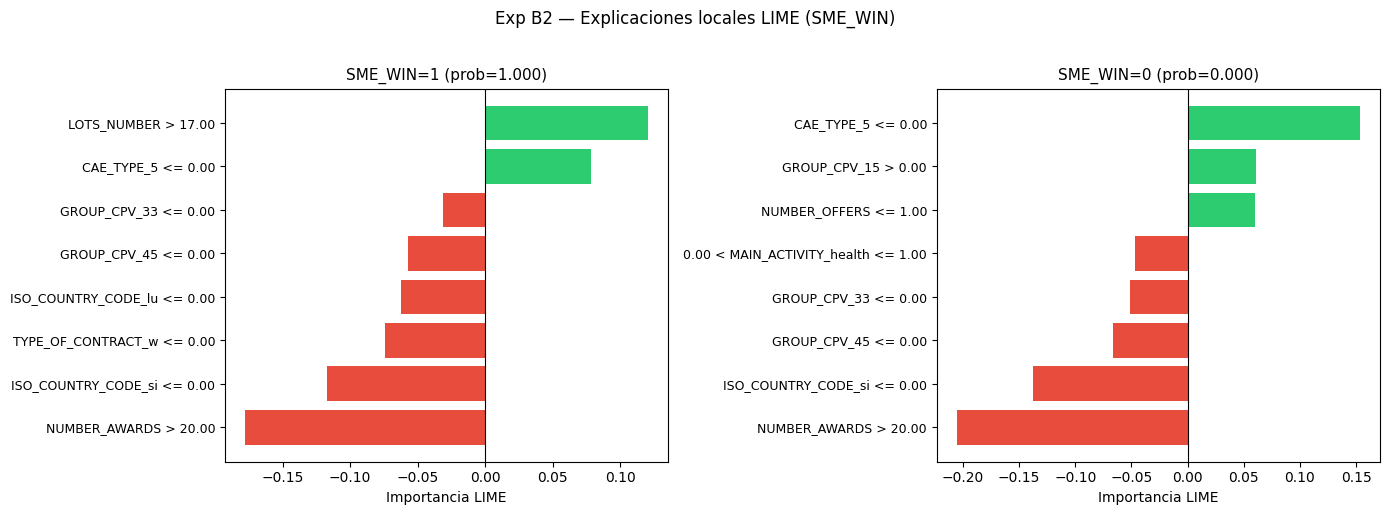
\includegraphics[width=\textwidth]{Imagenes/LIME_B2_instancias.png}
\caption{Explicaciones LIME para el Exp.~B2. Izquierda: SME\_WIN\,=\,1 (prob\,=\,1.000); derecha: SME\_WIN\,=\,0 (prob\,=\,0.000). Barras verdes favorecen, rojas penalizan.}
\label{fig:lime_b2_instancias}
\end{figure*}



\begin{figure*}[t]
%\begin{figure}[H]	
\centering

\includegraphics[width=\textwidth]{Imagenes/LIME_fidelidad.png}
\caption{Distribución del R\textsuperscript{2} de fidelidad LIME (50 instancias). Exp.~A: media 0.58, 45\,\% $>$0.85. Exp.~B2: media 0.16, 0\,\% $>$0.85.}
\label{fig:lime_fidelidad}
\end{figure*}



%\begin{figure}[htb]
\begin{figure*}[t]	
\centering
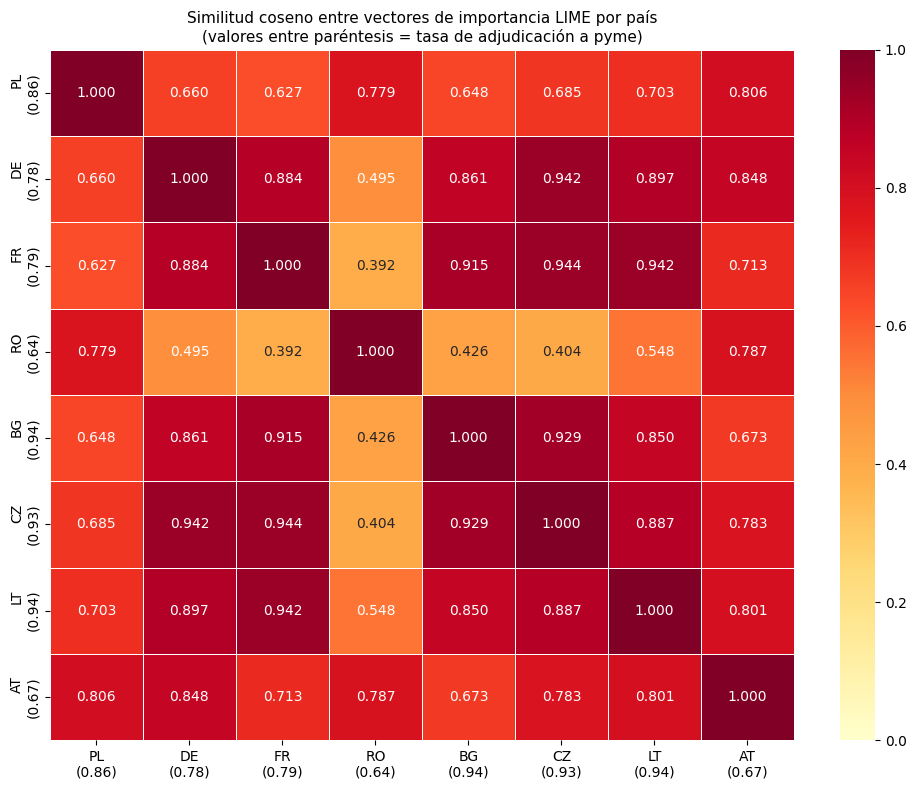
\includegraphics[width=0.75\textwidth]{Imagenes/LIME_consistencia_geografica.png}
\caption{Similitud coseno entre vectores de importancia LIME por país. FR--CZ: 0.944; DE--CZ: 0.942. RO es el país más atípico (sim promedio: 0.48).}
\label{fig:lime_geo}
\end{figure*}

 Estos resultados se pueden observar en las Figuras \ref{fig: XAI_RF_GA}, \ref{fig: XAI_GB_GA}, \ref{fig: XAI_RF_GB} y \ref{fig: XAI_GB_GB}.
 
 
 \paragraph{\textbf{Resultados de sistema de reglas y XAI para Experimento A.}}
	El Experimento A clasifica en base a la característica ``MAIN\_ACTIVITY'' aplicados en los dos modelos de ML. Las Figuras \ref{fig: XAI_RF_GA} y \ref{fig: XAI_GB_GA} muestran cómo los modelos toman las decisiones.
%
	En ambos casos, LIME destaca la relevancia de variables como \texttt{LOTS\_NUMBER}, \texttt{MAIN\_ACTIVITY\_health} y \texttt{TYPE\_OF\_CONTRACT}, reafirmando los patrones observados en la importancia de atributos.

 
 \begin{figure*}[t]
 	\caption{XAI para la primera clasificación}
 	\label{fig: XAI_RF_GA}
	\centering
 	
\includegraphics[width=1\linewidth]{Imagenes/capitulo_tres/GA/LIME_RF.png}

 \end{figure*}
 
 \begin{figure*}[t]
 	\caption{XAI para la segunda clasificación}
 	\label{fig: XAI_GB_GA}
	\centering
 	
\includegraphics[width=1\linewidth]{Imagenes/capitulo_tres/GA/LIME_GB.png}

 \end{figure*}
 
 \paragraph{\textbf{Resultados de sistema de reglas y XAI para Experimento B.}}
	El Experimento B clasifica en base a la característica  ``GROUP\_DURATION'' aplicados en los dos modelos de ML. Las Figuras \ref{fig: XAI_RF_GB} y \ref{fig: XAI_GB_GB} muestran las decisiones tomadas por los modelos.
 

 	En este experimento, LIME identifica como variables decisivas a \texttt{NUMBER\_OFFERS}, \texttt{NUMBER\_TENDERS\_SME} y \texttt{VALUE\_EURO}, lo que sugiere que la duración estimada del contrato está asociada a la competitividad del proceso y al monto económico involucrado.
 
 
 \begin{figure*}[t]
 	\caption{XAI para la primera clasificación}
 	\label{fig: XAI_RF_GB}
	\centering
 	
\includegraphics[width=1\textwidth]{Imagenes/capitulo_tres/GB/LIME_RF.png}

 \end{figure*}
 
 \begin{figure*}[t]
    \caption{XAI para la segunda clasificación}
     \label{fig: XAI_GB_GB}
   	\centering 	    
	 
\includegraphics[width=1\textwidth]{Imagenes/capitulo_tres/GB/LIME_GB.png}

 \end{figure*}
 
 
\section{Concluding remarks}

Este estudio presentó una metodología integral y reproducible para el análisis y la clasificación de licitaciones públicas europeas a partir de datos abiertos, combinando procesos de ingeniería de datos, modelos de aprendizaje automático supervisado y técnicas de inteligencia artificial explicable.
El enfoque propuesto demuestra la viabilidad de combinar análisis a gran escala con mecanismos de interpretación que facilitan la adopción de sistemas predictivos en contextos sensibles como la contratación pública.


\paragraph{\textbf{Data Collection / Data Requirements.}}
La construcción de un conjunto de datos normalizados a partir de fuentes públicas, mediante un flujo ETL escalable, se  garantizó la integración, limpieza y normalización de datos heterogéneos, garantizando una base consistente y reutilizable para el análisis posterior.


\paragraph{\textbf{Data Understanding.}}

El análisis exploratorio y estadístico del conjunto de datos facilitó la comprensión de la estructura, distribución y relaciones entre las variables más relevantes del proceso de contratación pública. Asimismo, permitió la identificación de desbalances de clase que influyen directamente en el rendimiento de los modelos predictivos. Estos resultados fueron muy importantes para orientar las etapas de preparación y evaluación de los modelos de clasificación.

\paragraph{\textbf{Modeling / Evaluation.}}

La implementación y evaluación de los modelos \textit{Random Forest} y \textit{Gradient Boosting} demostró que los enfoques basados en ensambles son adecuados para tareas de clasificación de licitaciones públicas. Bajo validación cruzada estratificada ($k=10$) sin fuga, RF supera a GB en ambos experimentos: F1\,=\,$0.3960 \pm 0.0124$ vs $0.3339 \pm 0.0104$ (Exp.~A); F1\,=\,$0.7706 \pm 0.0025$ y AUC\,=\,$0.7096 \pm 0.0050$ (Exp.~B2). RF es 31$\times$ más rápido en Exp.~A.

\paragraph{\textbf{Deployment.}}
Un aporte relevante de este trabajo es la integración de técnicas de inteligencia artificial explicable, en particular LIME, 
junto con \texttt{convert\_to\_if\_then()}, que presenta las importancias de LIME como reglas condicionales en lenguaje natural.
Esta combinación permitió interpretar localmente las decisiones de los modelos y vincular las predicciones con criterios comprensibles para analistas del dominio, fortaleciendo la transparencia y trazabilidad del sistema. De este modo, los resultados numéricos generados por los modelos de aprendizaje automático pueden ser contextualizados dentro del proceso de toma de decisiones en contratación pública.


\paragraph{\textbf{Feedback.}}
Finalmente, la fase de retroalimentación permitió consolidar los aprendizajes derivados del comportamiento del sistema y cerrar el ciclo de la metodología fundamental. En conjunto, los resultados confirman que la metodología propuesta constituye una base sólida para el desarrollo de sistemas de apoyo a la toma de decisiones en contratación pública, al articular datos abiertos, modelos predictivos y explicabilidad. Como líneas de trabajo futuro, se plantea la incorporación de estrategias avanzadas de balanceo, el análisis de métricas agregadas por clase y la evaluación del sistema en entornos operativos reales, con el fin de mejorar el rendimiento en clases minoritarias y reforzar su aplicabilidad práctica.


\paragraph{\textbf{Data and Code Availability..}}
Con el fin de garantizar la reproducibilidad de los resultados, todos los scripts de preprocesamiento de datos, los modelos entrenados y los recursos experimentales utilizados en este estudio se encuentran disponibles públicamente en:
%
\url{https://github.com/acuencao/tenders}.

\begin{figure*}[t]
\centering
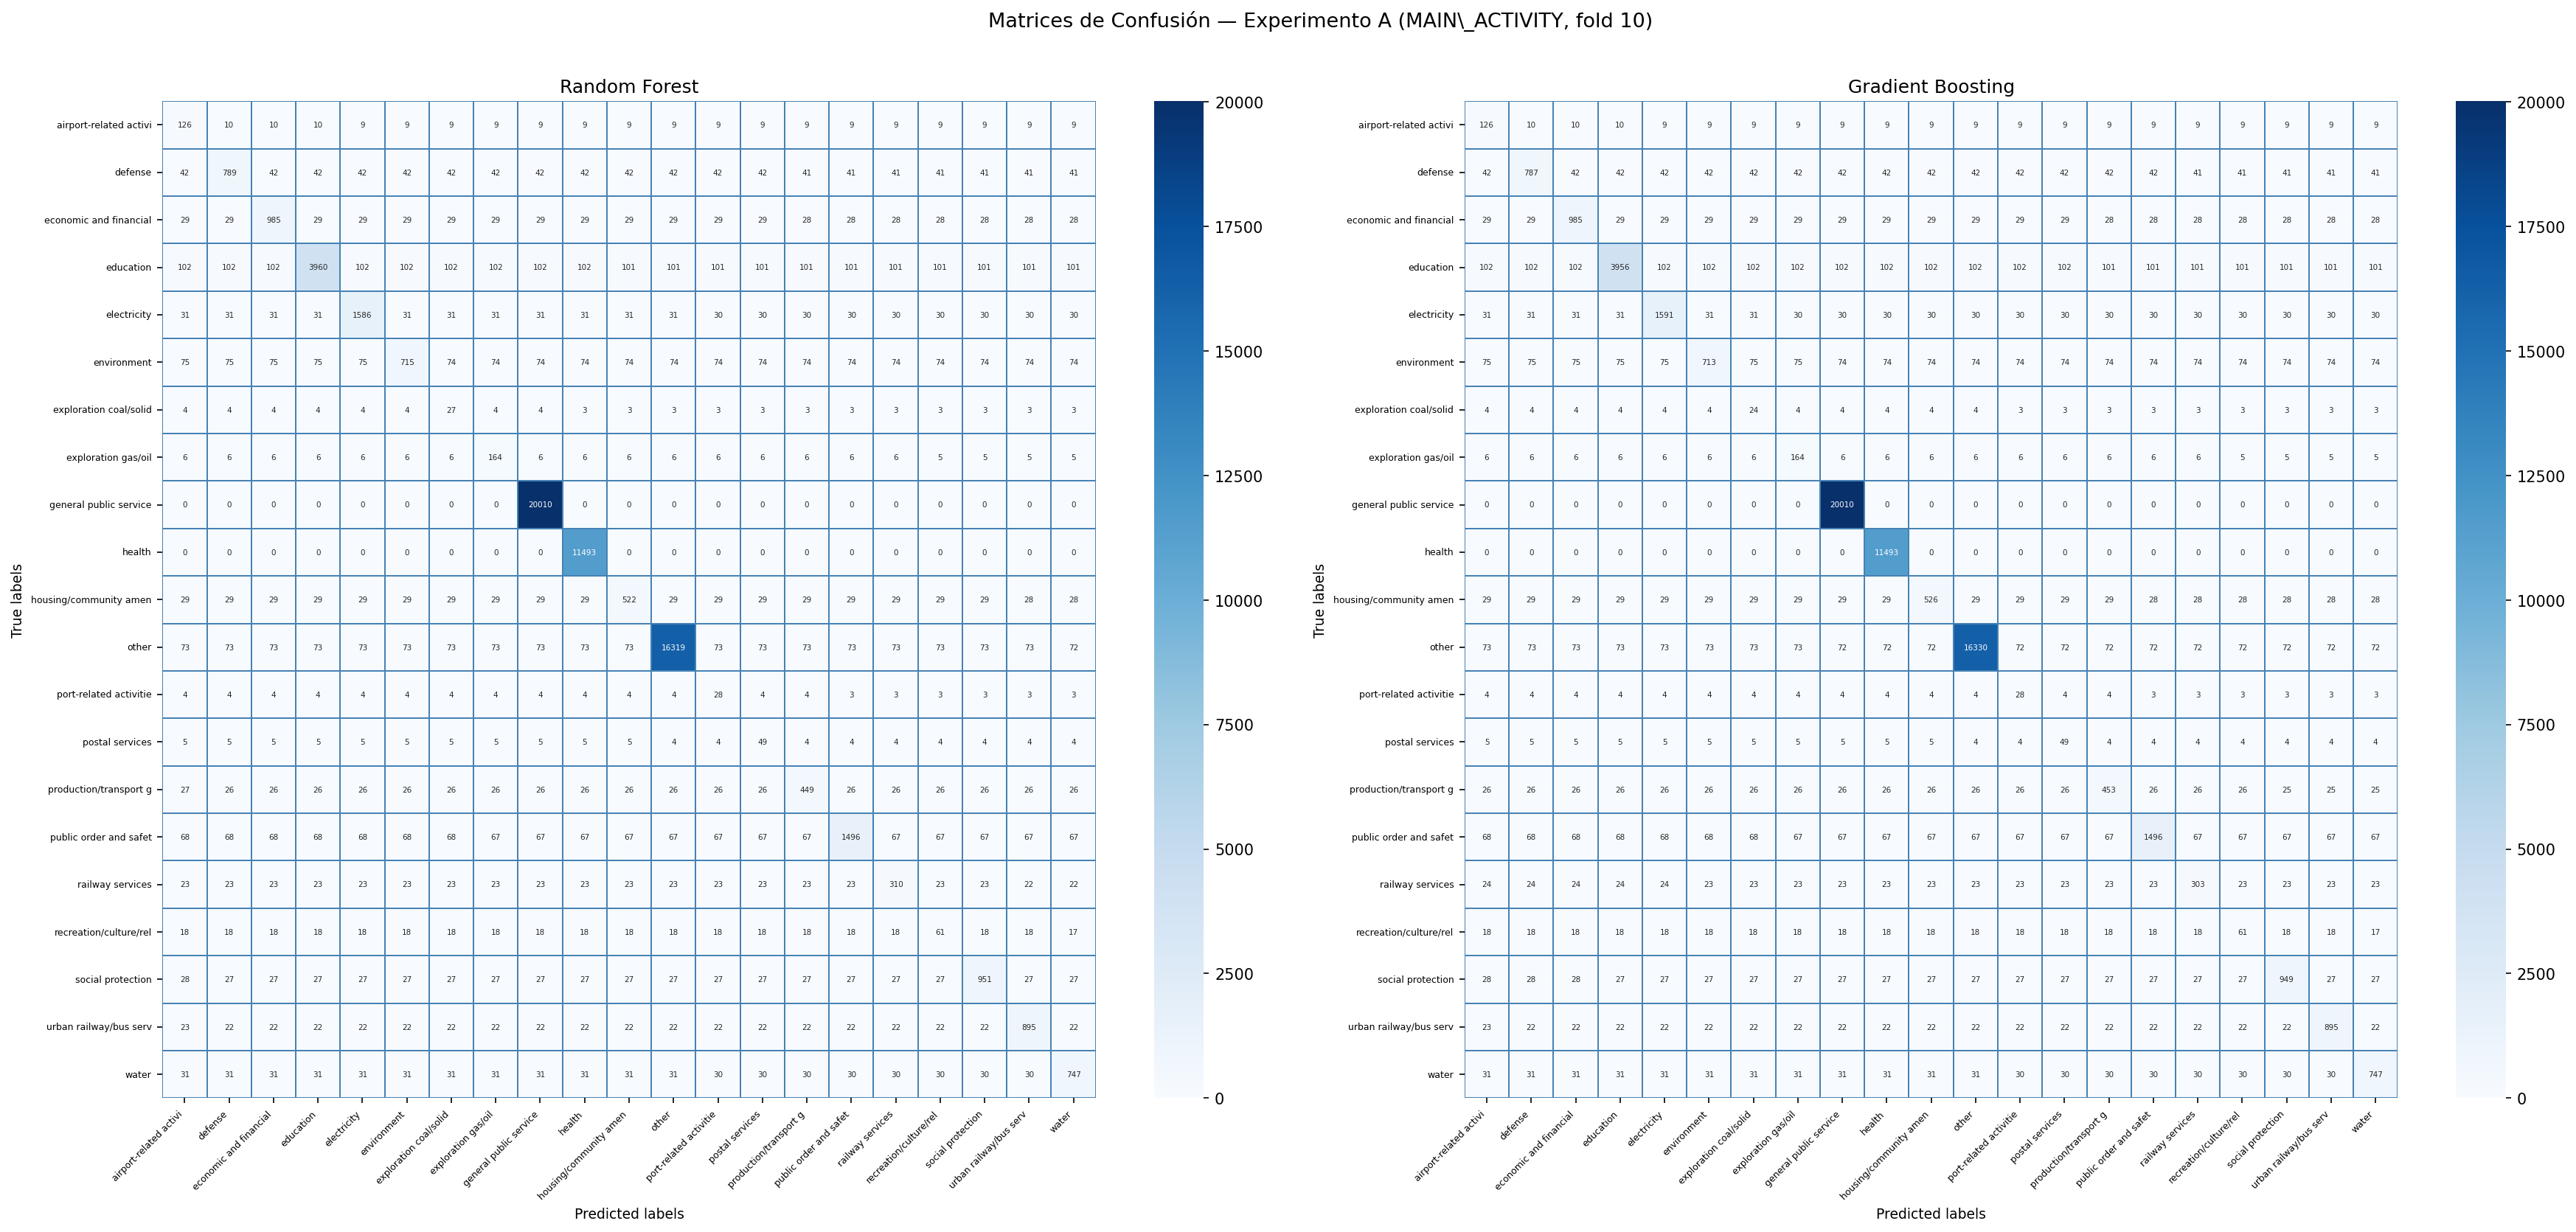
\includegraphics[width=\textwidth]{Imagenes/CM_ExpA_combinada.png}
\caption{Matrices de confusi\'on de los modelos Random Forest y Gradient Boosting para el Experimento~A (\texttt{MAIN\_ACTIVITY}, fold~10 de la validaci\'on cruzada estratificada $k=10$). Las clases \textit{general public services} y \textit{health} presentan las diagonales m\'as prominentes, reflejando su mayor representaci\'on en el conjunto de datos.}
\label{fig:cm_expA}
\end{figure*}

\begin{figure*}[t]
\centering
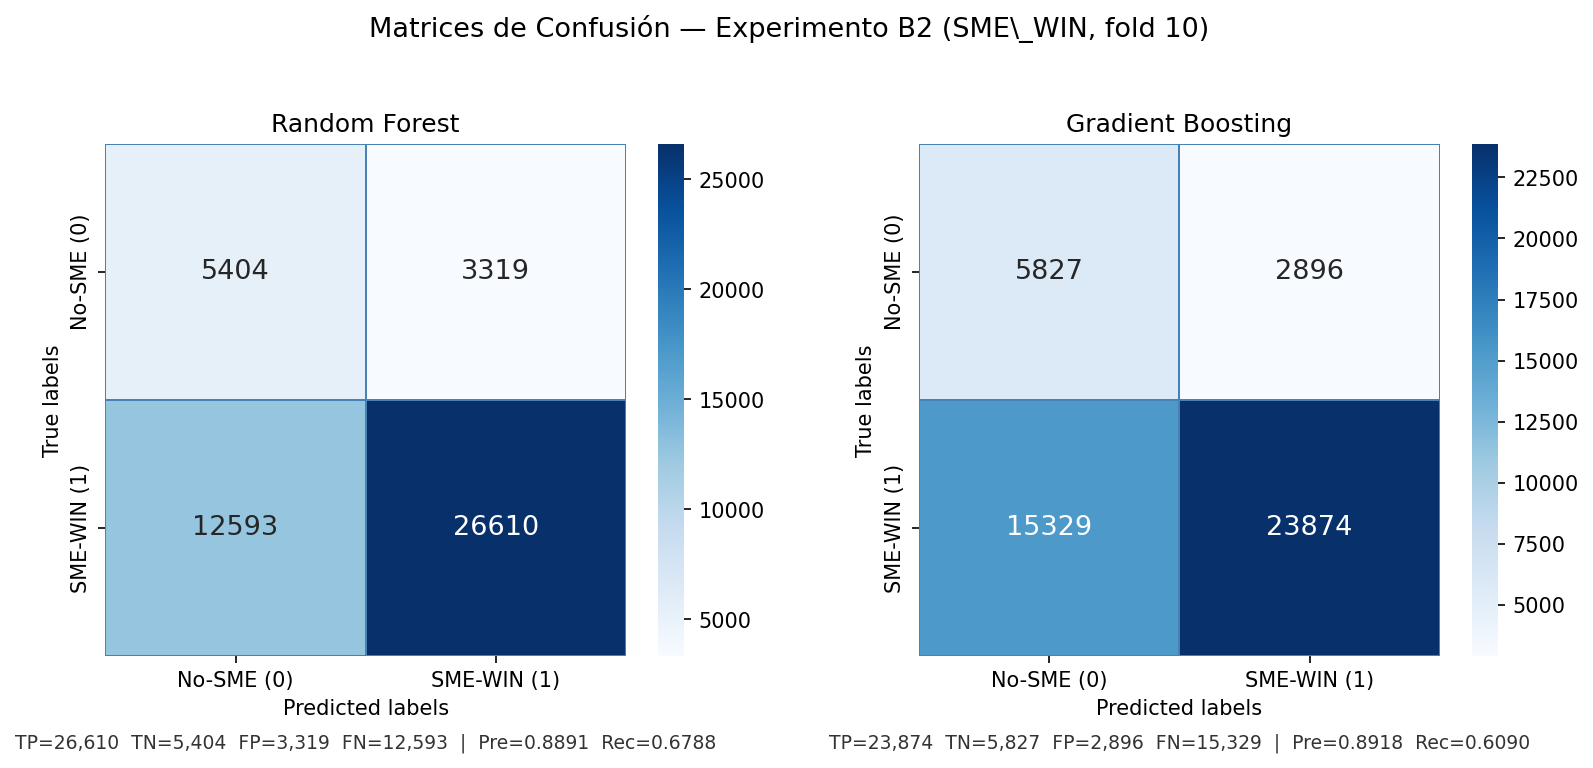
\includegraphics[width=\textwidth]{Imagenes/CM_ExpB2_combinada.png}
\caption{Matrices de confusi\'on de los modelos Random Forest y Gradient Boosting para el Experimento~B2 (\texttt{SME\_WIN}, fold~10). RF detecta m\'as verdaderos positivos (TP\,=\,26{,}610) que GB (TP\,=\,23{,}874) con una tasa de recall superior (68.1\,\% vs 60.9\,\%), confirmando su ventaja en la identificaci\'on de licitaciones favorables para pymes.}
\label{fig:cm_expB2}
\end{figure*}
\clearpage


%% Estilo bibliográfico de Elsevier (nombre-año). Alternativa numérica: model1-num-names
\bibliographystyle{cas-model2-names}
%\bibliography{biblio}

\end{document}
